%% ============================================================
%%  FULL RESTRUCTURED THESIS — XeLaTeX
%%  Title: Design and Implementation of an Automatic and
%%         Intelligent IT Resource Provisioning Solution
%%  Authors: HAMMAL Zakaria, SELATENIA Oussama,
%%           MENNOUR Oussama, DJEHA Younes
%%  Supervisor: Mr. Khaled ZERAOULIA
%%  Institution: USTHB — Faculty of Informatics
%% ============================================================

\documentclass[12pt,a4paper]{report}

% ── Core packages ────────────────────────────────────────────
\usepackage{fontspec}
\usepackage{geometry}
\usepackage{graphicx}
\usepackage{fancyhdr}
\usepackage{setspace}
\usepackage{tocloft}
\usepackage{titlesec}
\usepackage{amsmath}
\usepackage{amssymb}
\usepackage{array}
\usepackage{booktabs}
\usepackage{longtable}
\usepackage{tabularx}
\usepackage{caption}
\usepackage[linesnumbered,ruled,vlined]{algorithm2e}
\captionsetup{font=small, labelfont=bf, margin=1cm}

% ── Arabic / bilingual support ───────────────────────────────
\usepackage{polyglossia}
\setmainlanguage{english}
\setotherlanguage{arabic}
\newfontfamily\arabicfont[Script=Arabic]{Amiri}

% ── hyperref last ────────────────────────────────────────────
\usepackage{hyperref}
\hypersetup{
    colorlinks=true,
    linkcolor=black,
    citecolor=blue,
    urlcolor=blue,
}

% ── Widow / orphan control ───────────────────────────────────
\clubpenalty=10000
\widowpenalty=10000
\displaywidowpenalty=10000

% ── Page geometry ────────────────────────────────────────────
\geometry{left=3cm, right=2.5cm, top=2.5cm, bottom=2.5cm}

% ── Line spacing ─────────────────────────────────────────────
\onehalfspacing

% ── Header / footer ──────────────────────────────────────────
\pagestyle{fancy}
\fancyhf{}
\fancyhead[L]{\leftmark}
\fancyhead[R]{\thepage}
\renewcommand{\headrulewidth}{0.4pt}
\renewcommand{\footrulewidth}{0pt}

\fancypagestyle{plain}{%
  \fancyhf{}%
  \fancyhead[L]{\leftmark}%
  \fancyhead[R]{\thepage}%
  \renewcommand{\headrulewidth}{0.4pt}%
  \renewcommand{\footrulewidth}{0pt}%
}

% ── Chapter / section formatting ─────────────────────────────
\titleformat{\chapter}[display]
  {\normalfont\huge\bfseries}{\chaptertitlename\ \thechapter}{20pt}{\Huge}
\titlespacing*{\chapter}{0pt}{-20pt}{40pt}

% ── Convenience column type ──────────────────────────────────
\newcolumntype{L}[1]{>{\raggedright\arraybackslash}p{#1}}
\newcolumntype{C}[1]{>{\centering\arraybackslash}p{#1}}

% ============================================================
\begin{document}
% ============================================================

% ────────────────────────────────────────────────────────────
%  COVER PAGE
% ────────────────────────────────────────────────────────────
\newgeometry{left=2.5cm, right=2.5cm, top=1.5cm, bottom=1.5cm}
\begin{titlepage}
\thispagestyle{empty}
\centering

\vspace*{-1cm}

{\footnotesize Democratic and People's Republic of Algeria}\\
{\footnotesize \textarabic{الجمهورية الجزائرية الديمقراطية الشعبية}}

{\footnotesize Ministry of Higher Education and Scientific Research}\\
{\footnotesize \textarabic{وزارة التعليم العالي و البحث العلمي}}

\vspace{0.2cm}
\rule{\textwidth}{0.3pt}
\vspace{0.2cm}

\begin{minipage}{0.25\textwidth}
\centering

\includegraphics[width=0.9\textwidth]{usthb.png}
\end{minipage}
\hfill
\begin{minipage}{0.7\textwidth}
\centering
{\footnotesize \textarabic{جامعة العلوم والتكنولوجيا هواري بومدين}}\\
{\footnotesize University of Science and Technology Houari Boumediene}
\end{minipage}

\vspace{0.4cm}

{\LARGE \textbf{Faculty of Informatics}}\\
\vspace{0.4cm}
{\normalsize Thesis for graduation}\\
{\normalsize for the obtainment of the Bachelor degree}\\
\vspace{0.3cm}
{\normalsize \textbf{Option: ACAD}}

\vspace{0.3cm}
\rule{\textwidth}{0.6pt}
\vspace{0.3cm}

{\large \textbf{Design and Implementation of an Automatic and Intelligent IT Resource
Provisioning Solution (Servers and Virtual Machines) for the Scalable Deployment
of a High-Load Web Application.}}

\vspace{0.3cm}
\rule{\textwidth}{0.6pt}
\vspace{0.3cm}

\begin{minipage}{0.45\textwidth}
\normalsize \textit{Realized by:}\\
Mr.~Zakaria \textsc{Hammal}\\
Mr.~Oussama \textsc{Selatenia}\\
Mr.~Oussama \textsc{Mennour}\\
Mr.~Younes \textsc{Djeha}
\end{minipage}
\hfill
\begin{minipage}{0.45\textwidth}
\normalsize \textit{Supervised by:}\\
Mr.~Khaled \textsc{Zeraoulia}
\end{minipage}

\vspace{1cm}

{\normalsize Held on [DATE], before the jury composed of:}

{\normalsize Mr.~\textsc{Lastname} Firstname \hspace{0.5cm} -- President of jury}\\
{\normalsize Mr.~\textsc{Lastname} Firstname \hspace{0.5cm} -- Examiner}

\vspace{0.8cm}

{\normalsize Promotion: [YEAR/YEAR]}\\
{\normalsize Code PFE: [CODE]}

\end{titlepage}
\restoregeometry

% ============================================================
%  FRONT MATTER — Roman numerals
% ============================================================
\pagenumbering{roman}

% ────────────────────────────────────────────────────────────
%  DEDICATION
% ────────────────────────────────────────────────────────────
\newpage
\chapter*{Dedication}
\addcontentsline{toc}{chapter}{Dedication}
\thispagestyle{empty}

\vspace{1.5cm}

{\large ``}

\begin{center}
\itshape
To our families, whose patience and encouragement sustained this work through its
most demanding stages.\\[0.6cm]
To our mothers, our fathers, our brothers and sisters — your sacrifices made ours
possible.\\[0.6cm]
To every colleague who shared ideas, debugged midnight sessions, and believed in
this project.\\[0.8cm]
Thank you.
\end{center}

\begin{flushright}
{\large ''}
\end{flushright}

\vfill
\noindent\textbf{\textit{The Authors}}

% ────────────────────────────────────────────────────────────
%  ACKNOWLEDGEMENTS
% ────────────────────────────────────────────────────────────
\chapter*{Acknowledgements}
\addcontentsline{toc}{chapter}{Acknowledgements}

\vspace{0.5cm}

First and foremost, we render thanks to Allah, the Almighty, for granting us the
strength, patience, and clarity of mind required to bring this work to completion.

We express our profound gratitude to our supervisor, \textbf{Mr.~Khaled Zeraoulia},
for his invaluable guidance, availability, and constructive criticisms throughout
the elaboration of this project. His technical acumen and pedagogical approach were
decisive in shaping the rigour of this work.

We extend sincere thanks to the members of the jury for the honour they bestow upon
us by dedicating time to evaluate and enrich this thesis.

Finally, we acknowledge the contributions, direct and indirect, of the teaching staff
of the Faculty of Informatics at the University of Science and Technology Houari
Boumediene (USTHB), whose courses furnished the theoretical foundations upon which
this work is built.

% ────────────────────────────────────────────────────────────
%  ABSTRACT
% ────────────────────────────────────────────────────────────
\chapter*{Abstract}
\addcontentsline{toc}{chapter}{Abstract}

\vspace{0.5cm}

Modern healthcare information systems impose stringent requirements on their
underlying infrastructure: continuous availability, elastic scalability under
unpredictable load, and strict inter-tenant isolation. This thesis presents the
design and implementation of an autonomous, intelligent resource provisioning
framework for a cluster hosting a distributed medical information system.

The infrastructure is structured across four hierarchical layers: physical hardware,
virtualisation, container orchestration, and an overarching observability stratum. At
the virtualisation tier, a hybrid placement algorithm combining the Whale Optimisation
Algorithm (WOA) and Differential Evolution (DE) governs the mapping of virtual machines
to physical hosts, optimising a multi-objective fitness function that minimises CPU,
RAM, I/O, and energy resource gaps in a single weighted objective. Container scheduling within virtual
machine fleets is directed by a Best-Fit heuristic designed to maximise bin packing
efficiency and reduce fragmentation. Automated scaling --- both vertical and horizontal
--- is driven by telemetry-derived alerts with configurable severity thresholds.

An artificial intelligence layer augments rule-based orchestration with a gradient
boosted predictive model (XGBoost) that dynamically recalibrates the placement
algorithm's fitness weights according to the cluster's current structural bottleneck.
A dual-agent cognitive system, composed of a Planner and an independent Critic,
executes remediation actions under a risk-based escalation policy. Low- and
medium-risk actions are executed autonomously; high-risk operations are deferred to
an administrator via an asynchronous email approval workflow, with the entire decision
chain recorded in an immutable audit log.

The system is evaluated in a proof-of-concept deployment of a microservices-based
medical information system comprising ministry- and hospital-tier services, partitioned
into five logically isolated Kubernetes namespaces and three network segments.

\vspace{1.2cm}
\noindent\rule{\textwidth}{0.4pt}\\[4pt]
\noindent\textbf{Keywords:} cloud computing, virtualisation, container orchestration,
microservices, Whale Optimisation Algorithm, Differential Evolution, Kubernetes,
Prometheus, autonomous provisioning, AI-driven orchestration.\\[4pt]
\noindent\rule{\textwidth}{0.4pt}

\vspace{1.5cm}

\noindent\textbf{Résumé}

\vspace{0.3cm}

Les systèmes d'information de santé modernes imposent des contraintes sévères à leur
infrastructure : disponibilité continue, scalabilité élastique et isolation stricte
entre locataires. Ce mémoire présente la conception et la réalisation d'un cadre
autonome et intelligent de provisioning de ressources pour un cluster hébergeant un
système d'information médical distribué.

L'infrastructure est structurée en quatre couches hiérarchiques. Un algorithme hybride
WOA-DE gouverne le placement des machines virtuelles sur les hôtes physiques en
minimisant une fonction de fitness multi-objectif. L'ordonnancement des conteneurs est
assuré par une heuristique Best-Fit. Un modèle XGBoost recalibre dynamiquement les
poids du placement selon le goulot d'étranglement courant du cluster. Un système
dual-agent (Planificateur / Critique) exécute les actions de remédiation sous une
politique d'escalade fondée sur le risque.

\vspace{0.8cm}
\noindent\rule{\textwidth}{0.4pt}\\[4pt]
\noindent\textbf{Mots-clés :} virtualisation, orchestration de conteneurs,
microservices, Whale Optimisation Algorithm, Differential Evolution, Kubernetes,
Prometheus, provisioning autonome, orchestration par IA.\\[4pt]
\noindent\rule{\textwidth}{0.4pt}

% ────────────────────────────────────────────────────────────
%  TABLE OF CONTENTS / FIGURES / TABLES
% ────────────────────────────────────────────────────────────
\tableofcontents
\newpage

\listoffigures
\addcontentsline{toc}{chapter}{List of Figures}
\newpage

\listoftables
\addcontentsline{toc}{chapter}{List of Tables}
\newpage

% ============================================================
%  MAIN MATTER — Arabic numerals
% ============================================================
\pagenumbering{arabic}
\setcounter{page}{1}

% ============================================================
%  GENERAL INTRODUCTION
% ============================================================
\chapter*{General Introduction}
\addcontentsline{toc}{chapter}{General Introduction}
\markboth{GENERAL INTRODUCTION}{GENERAL INTRODUCTION}

The progressive digitisation of critical public services --- healthcare in particular ---
has imposed unprecedented demands on the software infrastructures that underpin them.
A regional health information system must coordinate diagnostic records, pharmaceutical
prescriptions, inter-hospital referrals, and administrative workflows across a
geographically dispersed set of institutions, often under time-sensitive conditions
where a processing delay translates directly into degraded patient care. These
operational constraints place scalability, fault tolerance, and security at the centre
of any credible technical design.

The emergence of virtualisation and container orchestration technologies has
fundamentally altered the economics and operational logic of such infrastructures.
Where previously a dedicated physical server was required for each application
service, a modern cluster can consolidate hundreds of isolated workloads onto a
shared hardware fleet, responding dynamically to load fluctuations without human
intervention. Yet this operational flexibility is not freely obtained. Distributed
systems introduce complexity that static provisioning models cannot address: an
improperly placed workload propagates resource contention; a rigidly defined alert
threshold fires at the wrong granularity; and a naive scaling trigger may inadvertently
amplify the failure it was designed to contain.

This thesis investigates the architectural and algorithmic means by which this
complexity can be brought under intelligent, automated control. The central question
is the following: how can a cluster infrastructure spanning physical hardware,
virtualisation, and container orchestration both maximise resource
efficiency and guarantee continuous service availability for a high-load distributed
application, while maintaining a security posture compatible with sensitive health
data?

To address this question, three primary objectives were pursued. The first is to
design a hierarchical, layer-separating cluster architecture that establishes explicit
failure domains and network isolation boundaries without sacrificing operational
flexibility. The second is to develop and integrate a multi-objective optimisation
algorithm --- the hybrid WOA-DE --- that governs virtual machine placement with
awareness of CPU, RAM, I/O, and energy constraints within a single fitness objective. The third is to
build an autonomous orchestration layer, grounded in machine learning and dual-agent
reasoning, capable of detecting emerging resource pathologies and executing calibrated
remediation actions within a risk-bounded decision policy.

The document is organised as follows. Chapter~1 surveys the state of the art across
the relevant domains: hardware virtualisation models, containerisation architectures,
container orchestration platforms, and prior work on virtual machine placement
algorithms, situating the present contribution within the existing literature.
Chapter~2 presents the general conceptual design of the proposed infrastructure in a
technology-agnostic manner, articulating the four-layer architectural model, the
WOA-DE placement algorithm and its fitness function, the monitoring and alert
management subsystem, and the dual-agent AI framework with its associated security
constraints. Chapter~3 grounds this design in a concrete implementation, documenting
the specific technology choices made at each architectural layer and describing the
deployed medical information system that serves as the proof-of-concept workload.
Unavoidably, Chapter~3 remains partially incomplete at the time of writing, pending
finalisation of the deployment environment; all such gaps are explicitly labelled.

% ============================================================
%  CHAPTER 1 — STATE OF THE ART
% ============================================================
\chapter{State of the Art}

\section{Introduction}

Virtualised, containerised infrastructure management has generated a substantial
research literature over the past two decades, spanning hypervisor engineering,
container runtime design, distributed orchestration, and combinatorial resource
allocation. Surveying this body of work is not merely a formality: the specific
design decisions in Chapter~2 --- the choice of a hybrid placement strategy, the
three-segment network model, the two-tier agent architecture --- each respond to
identifiable shortcomings in prior approaches. This chapter maps those shortcomings
through structured comparative analyses of the relevant technology families and closes
with a critical synthesis that locates the precise gap this thesis addresses.

% ─────────────────────────────────────────────────────────────────
\section{Hardware Virtualisation}

\subsection{Hypervisor Classification}

Two primary hypervisor architectures govern the landscape of hardware virtualisation.
Type~1 hypervisors --- often termed bare-metal hypervisors --- execute directly on
the physical hardware without an intervening host operating system. This direct
hardware access yields lower scheduling latency and higher throughput. Type~2
hypervisors run as processes within a conventional host operating system, trading
raw performance for installation simplicity and portability. Table~\ref{tab:hypervisors}
contrasts the defining characteristics of each class.

\begin{table}[htbp]
\centering
\caption{Comparative analysis of Type~1 and Type~2 hypervisors.}
\label{tab:hypervisors}
\begin{tabular}{L{3.2cm} L{5.5cm} L{5.5cm}}
\toprule
\textbf{Criterion} & \textbf{Type 1 (Bare-Metal)} & \textbf{Type 2 (Hosted)} \\
\midrule
Execution layer     & Directly on hardware; no host OS & As a process within a host OS \\
\addlinespace
Performance         & Near-native; minimal overhead & Additional OS scheduling layer \\
\addlinespace
Security isolation  & Strong; no shared host OS kernel & Weaker; host compromise affects all guests \\
\addlinespace
Typical use case    & Production data centres, enterprise deployments & Developer workstations, testing environments \\
\addlinespace
Examples            & VMware ESXi, Microsoft Hyper-V, Xen, KVM, Proxmox VE & VirtualBox, VMware Workstation, QEMU (user mode) \\
\addlinespace
Hardware access     & Direct, via device drivers in hypervisor & Via host OS device driver stack \\
\addlinespace
Deployment cost     & High; requires dedicated hardware & Low; runs on existing hardware \\
\bottomrule
\end{tabular}
\end{table}

\subsection{Virtual Machines versus Containers}

Virtual machines and containers both deliver workload isolation, yet they operate at
fundamentally different levels of the system stack. A virtual machine encapsulates an
entire operating system, whereas a container shares the host kernel and isolates only
the user-space environment. Table~\ref{tab:vm_vs_container} presents the principal
trade-offs between these two paradigms.

\begin{table}[htbp]
\centering
\caption{Virtual machines versus containers: a comparative analysis.}
\label{tab:vm_vs_container}
\begin{tabular}{L{3.2cm} L{5.5cm} L{5.5cm}}
\toprule
\textbf{Criterion} & \textbf{Virtual Machines} & \textbf{Containers} \\
\midrule
Isolation unit      & Full guest OS + application & Process namespaces + cgroups \\
\addlinespace
Startup time        & Tens of seconds to minutes & Sub-second to a few seconds \\
\addlinespace
Image size          & Gigabytes (full OS) & Megabytes to a few hundred MB \\
\addlinespace
Kernel sharing      & Independent kernel per VM & Shared host kernel \\
\addlinespace
Security boundary   & Strong hardware-enforced boundary & Weaker; kernel vulnerabilities affect all \\
\addlinespace
Resource overhead   & High (hypervisor + guest OS) & Low (thin runtime layer) \\
\addlinespace
Density per host    & Tens of VMs per host & Hundreds of containers per host \\
\addlinespace
Portability         & Image-level (OVA, VMDK) & Image-level (OCI/Docker) \\
\addlinespace
Persistent storage  & Virtual disk files & Volumes external to container \\
\bottomrule
\end{tabular}
\end{table}

\begin{figure}[htbp]
\centering
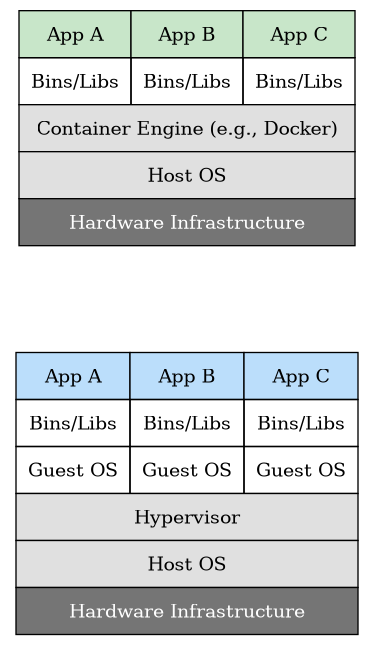
\includegraphics[width=0.85\linewidth, keepaspectratio]{arch_vm_container.gv.png}
\caption{Architectural comparison between hardware virtualisation (Virtual Machines)
and operating-system-level virtualisation (Containers).
Source: adapted from open documentation.}
\label{fig:vm_vs_container}
\end{figure}

% ─────────────────────────────────────────────────────────────────
\section{Software Architecture: Monolithic vs Microservices}

The structural design of the application layer profoundly conditions the scalability
of the underlying infrastructure. A monolithic application consolidates all business
logic, data access layers, and interface components into a single deployable artefact.
A microservices architecture, by contrast, decomposes the application into a collection
of autonomous services, each encapsulating a single bounded business capability and
communicating via well-defined interfaces. Table~\ref{tab:mono_micro} summarises the
operational trade-offs between these two paradigms.

\begin{table}[htbp]
\centering
\caption{Monolithic architecture versus microservices: comparative analysis.}
\label{tab:mono_micro}
\begin{tabular}{L{3.2cm} L{5.5cm} L{5.5cm}}
\toprule
\textbf{Criterion} & \textbf{Monolithic} & \textbf{Microservices} \\
\midrule
Scalability         & Entire application replicated; coarse-grained & Per-service scaling; fine-grained \\
\addlinespace
Deployment          & Single artefact; atomic but risky & Independent per-service deployments \\
\addlinespace
Fault isolation     & Single point of failure for all functions & Graceful degradation; faults contained \\
\addlinespace
Technology stack    & Uniform across entire codebase & Polyglot; per-service choice \\
\addlinespace
Inter-module coupling & Tight; function calls within process & Loose; network API contracts \\
\addlinespace
Operational complexity & Low; single process to monitor & High; distributed tracing required \\
\addlinespace
Release velocity    & Slows as codebase grows & High; independent release cycles \\
\addlinespace
Data management     & Single shared database & Database-per-service pattern \\
\addlinespace
Team structure      & Centralised; all teams share codebase & Autonomous teams per service \\
\bottomrule
\end{tabular}
\end{table}

% ─────────────────────────────────────────────────────────────────
\section{Container Orchestration Platforms}

As the number of containerised services grows beyond the capacity of manual
administration, orchestration platforms become essential. Table~\ref{tab:orchestration}
compares the three principal open-source container orchestration systems.

\begin{table}[htbp]
\centering
\caption{Comparison of leading container orchestration platforms.}
\label{tab:orchestration}
\begin{tabular}{L{2.8cm} L{3.8cm} L{3.8cm} L{3.8cm}}
\toprule
\textbf{Criterion} & \textbf{Kubernetes} & \textbf{Docker Swarm} & \textbf{HashiCorp Nomad} \\
\midrule
Architecture        & Control plane + worker nodes; etcd state store & Manager + worker nodes; Raft consensus & Client-server; Raft consensus \\
\addlinespace
Workload types      & Containers, Jobs, StatefulSets, DaemonSets & Services, Tasks & Containers, JVM apps, scripts \\
\addlinespace
Auto-scaling        & HPA, VPA, KEDA & Manual or external & Autoscaler via external plugin \\
\addlinespace
Networking          & CNI plugins (Calico, Flannel, Cilium) & Overlay (VXLAN-based) & CNI plugins \\
\addlinespace
Storage             & PersistentVolume / StorageClass abstractions & Volume mounts & Host volumes, CSI plugins \\
\addlinespace
Learning curve      & High & Low to medium & Medium \\
\addlinespace
Community maturity  & Very high; CNCF flagship & Declining; Docker-native & Growing \\
\addlinespace
Multi-tenancy       & Namespaces + RBAC + NetworkPolicy & Stack isolation only & Namespaces + ACL \\
\bottomrule
\end{tabular}
\end{table}

% ─────────────────────────────────────────────────────────────────
\section{Virtualisation Platforms}

The choice of virtualisation platform determines the capabilities available for
VM lifecycle management, high availability, and integration with the orchestration
layer above it. Table~\ref{tab:virt_platforms} compares the leading open-source and
commercial alternatives.

\begin{table}[htbp]
\centering
\caption{Comparison of virtualisation platforms.}
\label{tab:virt_platforms}
\begin{tabular}{L{2.8cm} L{3.5cm} L{3.5cm} L{3.5cm}}
\toprule
\textbf{Criterion} & \textbf{Proxmox VE} & \textbf{VMware vSphere} & \textbf{OpenStack} \\
\midrule
Licence             & Open-source (AGPL) with enterprise subscription option & Proprietary; per-socket licensing & Open-source (Apache 2.0) \\
\addlinespace
Hypervisor          & KVM (QEMU) + LXC & ESXi (proprietary) & KVM, Xen, HyperV (pluggable) \\
\addlinespace
Management UI       & Web-based; REST API & vCenter; REST API & Horizon dashboard; REST APIs \\
\addlinespace
Cluster features    & HA, live migration, shared storage, clustering & DRS, HA, vMotion, vSAN & Nova scheduling, live migration \\
\addlinespace
Storage integration & ZFS, Ceph, iSCSI, NFS, local LVM & vSAN, NFS, iSCSI, vVols & Cinder (block), Swift (object) \\
\addlinespace
Container support   & LXC natively; Docker via VMs & VMware Tanzu (additional cost) & Via Nova or Kubernetes integration \\
\addlinespace
On-premises suitability & Excellent; low cost & Excellent; high cost & Suitable for large deployments \\
\addlinespace
Learning curve      & Moderate & High & Very high \\
\bottomrule
\end{tabular}
\end{table}

% ─────────────────────────────────────────────────────────────────
\section{VM Placement Algorithms in the Literature}

Virtual machine placement constitutes a combinatorially complex optimisation problem
whose difficulty scales with the number of physical hosts, candidate VMs, and
optimisation objectives. Several algorithmic families have been explored in the
literature. Table~\ref{tab:placement_alg} presents a non-exhaustive review.

\begin{table}[htbp]
\centering
\caption{VM placement algorithms from the literature.}
\label{tab:placement_alg}
\begin{tabular}{L{2.5cm} L{3cm} L{4cm} L{4.2cm}}
\toprule
\textbf{Algorithm family} & \textbf{Examples} & \textbf{Optimisation objective} & \textbf{Key characteristics} \\
\midrule
Bin-packing heuristics & First-Fit, Best-Fit, Worst-Fit & Minimise active hosts & Fast; no convergence guarantee; greedy \\
\addlinespace
Evolutionary / genetic & GA, DE \cite{storn1997de} & Multi-objective resource utilisation & Population-based; good exploration; computationally heavier \\
\addlinespace
Swarm intelligence & PSO, WOA \cite{mirjalili2016woa}, Bat Algorithm & Energy + load balance & Bio-inspired; prone to premature convergence in isolation \\
\addlinespace
Reinforcement learning & DQN, PPO, CILP \cite{tuli2023cilp} & Long-horizon energy savings & Learns online; high training cost; hard to interpret \\
\addlinespace
Multi-criteria (AHP) & AHP-DRS \cite{gu2023towards} & Weighted multi-attribute scoring & Transparent weighting; expert knowledge required \\
\addlinespace
Hybrid (WOA + DE) & This work & CPU + RAM + I/O + energy & Combines exploitation depth (WOA) with diversity maintenance (DE) \\
\bottomrule
\end{tabular}
\end{table}

% ─────────────────────────────────────────────────────────────────
\section{Critical Synthesis: Open Problems in VM Placement}

The algorithm families surveyed in Table~\ref{tab:placement_alg} share a recurring
set of unresolved limitations that motivate the design decisions in Chapter~2.

\textit{Single-objective optimisation.} Bin-packing heuristics (First-Fit, Best-Fit)
minimise the count of active hosts but are blind to energy consumption and network
traffic patterns. Saxena et al. \cite{saxena2022secure} introduce security as a
second objective; Yang et al. \cite{yang2025task} add task structure; none integrates
CPU, RAM, I/O, and energy simultaneously under a normalised, dynamically weighted
objective. The fitness function proposed in Section~2.5 addresses this directly.

\textit{Premature convergence in isolation.} Pure WOA \cite{mirjalili2016woa}
concentrates the population around the current best solution within a few dozen
iterations on high-dimensional placement problems, where the search space grows
exponentially with the number of hosts. The convergence behaviour is well-documented
and is the primary motivation for hybridisation. DE \cite{storn1997de} avoids this
collapse through algebraic mutation but converges slowly on exploitation-heavy problems.
Neither algorithm alone is adequate for the time-sensitive provisioning loop of an
on-line cluster.

\textit{Static thresholds.} Even systems with sound placement algorithms --- including
Lai et al. \cite{lai2025energy} and Alahmad and Agarwal \cite{alahmad2024multiple} ---
rely on fixed resource thresholds to trigger migrations. Fixed thresholds assume
stationary workload distributions, an assumption that fails for microservices
deployments subject to diurnal traffic cycles and sudden load spikes. Saxena and Singh
\cite{saxena2022proactive} propose a neural network for dynamic threshold prediction
but provide no mechanism to recalibrate the placement fitness function accordingly.

\textit{Absence of safety-bounded autonomous execution.} The works reviewed address
placement and scaling as algorithmic problems, but none proposes a governance framework
for autonomous remediation. Tuli et al. \cite{tuli2023cilp} demonstrate online
learning for provisioning but treat execution as unrestricted; the consequences of an
incorrectly predicted action on a production cluster are not considered. The dual-agent
system with monotonic risk escalation developed in Section~2.8 is a direct response to
this gap.

\textit{Infrastructure-as-monolith assumption.} Most placement papers treat the
cluster as a flat pool of physical machines. The mini-cluster partitioning proposed
in Section~2.5 departs from this model: by partitioning the search space along
application dependency boundaries, scheduling complexity is reduced from $O(n)$ to
$O(n/k)$ and the majority of inter-service traffic is confined within a single
logical segment.

% ─────────────────────────────────────────────────────────────────
\section{Related Works}

Table~\ref{tab:related} synthesises the contributions most directly pertinent to the
present thesis. Each entry corresponds to a bibliographic reference cited in the
following chapters.

\begin{longtable}{L{2.2cm} C{1cm} L{3.2cm} L{2.8cm} L{2.5cm} L{2.8cm}}
\caption{Related works: synthesis table.}
\label{tab:related}\\
\toprule
\textbf{Authors} & \textbf{Year} & \textbf{Contribution} & \textbf{Methodology} & \textbf{Strengths} & \textbf{Limitations / Relevance} \\
\midrule
\endfirsthead
\multicolumn{6}{l}{\small\itshape Table~\ref{tab:related} continued\ldots}\\
\toprule
\textbf{Authors} & \textbf{Year} & \textbf{Contribution} & \textbf{Methodology} & \textbf{Strengths} & \textbf{Limitations / Relevance} \\
\midrule
\endhead
\midrule
\multicolumn{6}{r}{\small\itshape Continued on next page}\\
\endfoot
\bottomrule
\endlastfoot

Mirjalili \& Lewis \cite{mirjalili2016woa}
  & 2016
  & Introduces the Whale Optimisation Algorithm (WOA)
  & Bio-inspired; bubble-net hunting model
  & Strong exploitation; simple parameter set
  & Premature convergence; foundational reference for WOA component \\
\addlinespace

Storn \& Price \cite{storn1997de}
  & 1997
  & Differential Evolution for global optimisation
  & Population-based algebraic mutation and crossover
  & Excellent exploration; monotonic improvement
  & Requires continuous search space; provides DE component \\
\addlinespace

Zhang, Zhou \& Wang \cite{zhang2020intelligent}
  & 2020
  & Intelligent optimal VM allocation in cloud data centres
  & Multi-objective evolutionary optimisation
  & Demonstrated applicability to VM placement
  & Cloud-centric; limited energy awareness \\
\addlinespace

Saxena et al. \cite{saxena2022secure}
  & 2022
  & Secure and multi-objective VM placement framework
  & Multi-objective optimisation with security constraints
  & Combines performance and security objectives
  & Does not address AI-driven dynamic weight recalibration \\
\addlinespace

Saxena \& Singh \cite{saxena2022proactive}
  & 2022
  & Proactive autoscaling with neural network VM allocation
  & Online multi-resource neural network
  & Proactive approach; energy-efficient
  & Neural network interpretability limitations \\
\addlinespace

Alahmad \& Agarwal \cite{alahmad2024multiple}
  & 2024
  & Dynamic VM placement for application availability
  & Multi-objective dynamic placement in cloud networks
  & Availability-aware; dynamic adaptation
  & Does not handle on-premises cluster topology \\
\addlinespace

Tuli, Casale \& Jennings \cite{tuli2023cilp}
  & 2023
  & Co-simulation imitation learning for resource provisioning
  & Reinforcement learning via co-simulation
  & Handles dynamic environments; learns online
  & High training overhead; black-box decisions \\
\addlinespace

Senjab et al. \cite{senjab2023survey}
  & 2023
  & Survey of Kubernetes scheduling algorithms
  & Systematic literature review
  & Comprehensive overview of K8s scheduling
  & Survey only; no novel algorithm \\
\addlinespace

Lai, Zheng \& Lu \cite{lai2025energy}
  & 2025
  & Energy-aware VM migration with dual resource thresholds
  & Threshold-based live migration policy
  & Energy savings with performance guarantees
  & Dual-threshold approach; informs scaling thresholds \\
\addlinespace

Begam, Wang \& Zhu \cite{begam2020timer}
  & 2020
  & Time-sensitive VM provisioning in resource-constrained clouds
  & Bin-packing with time constraints
  & Addresses time-sensitive workloads
  & Limited multi-objective scope \\
\addlinespace

Yang et al. \cite{yang2025task}
  & 2025
  & Task-driven VM optimisation placement model
  & Task-aware placement optimisation
  & Task-specific resource allocation
  & Does not address AI-based dynamic adaptation \\
\addlinespace

Gu et al. \cite{gu2023towards}
  & 2023
  & Multi-decision AHP VM scheduling in cloud platforms
  & AHP-based multi-criteria scheduling
  & Transparent decision process; multi-criteria aware
  & Expert-dependent weight assignment \\
\addlinespace

Nguyen, Phan \& Kim \cite{nguyen2022load}
  & 2022
  & Load balancing of Kubernetes-based edge infrastructure
  & Resource-adaptive proxy for K8s edge clusters
  & Practical K8s load distribution
  & Edge-specific; limited to proxy layer \\
\addlinespace

Bompotas, Kalogeropoulos \& Makris \cite{bompotas2025commc}
  & 2025
  & Multi-purpose commodity hardware cluster design
  & Cluster architecture with commercial off-the-shelf hardware
  & Low-cost cluster feasibility
  & General purpose; no placement optimisation \\
\addlinespace

Balabanov \& Apostolov \cite{balabanov2025dcim}
  & 2025
  & Data centre infrastructure monitoring standards
  & DCIM methodology survey
  & Comprehensive monitoring taxonomy
  & Monitoring scope only; no placement \\
\addlinespace

Sung, Han \& Kim \cite{sung2024cloning}
  & 2024
  & VM pre-provisioning via cloning for edge cloud
  & Clone-based horizontal scaling
  & Fast horizontal scaling via snapshot cloning
  & Edge context; informs clone-based scaling strategy \\

\end{longtable}

\section{Conclusion}

Four structural gaps emerge from this review. First, no existing placement work
combines all four resource dimensions --- CPU, RAM, I/O, and energy --- under a
single normalised objective whose weights are recalibrated at runtime by a predictive
model; approaches addressing multiple objectives fix their weight vectors at design
time. Second, hybrid evolutionary strategies that combine WOA's exploitation
geometry with DE's population diversity consistently avoid the convergence failure
of single-paradigm bio-inspired optimisers, yet no published placement system applies
this combination to an on-premises, on-line provisioning scenario. Third, the
migration from static to dynamic alert thresholds has been studied at the
monitoring layer but not connected back to the placement layer: no system feeds
predicted bottleneck classifications into a placement fitness recalibration loop.
Fourth, autonomous remediation in production clusters has been demonstrated only
without governance constraints; the question of how to bound an agent's authority
to prevent irreversible damage has not been formally addressed.

The architecture proposed in Chapter~2 targets precisely these four gaps. The
WOA-DE hybrid eliminates premature convergence at the placement layer. The
multi-objective weighted Euclidean fitness with Z-score normalisation integrates all
four resource dimensions. The XGBoost prediction layer feeds dynamically adjusted
weights back to the placement algorithm. The Planner/Critic dual-agent system with
monotonic risk escalation provides autonomous execution with bounded authority. The
experimental system described in Chapter~3 constitutes the first integrated
realisation of all four mechanisms on a single on-premises cluster.


% ============================================================
%  CHAPTER 2 — CONCEPTION (technology-agnostic)
% ============================================================
\chapter{Conception}

\section{Introduction}

A cluster capable of sustaining a high-load distributed application under the
competing imperatives of resource efficiency and continuous availability cannot be
designed at a single abstraction level. Decisions at the hardware layer constrain
what the virtualisation layer can offer; those decisions constrain what the container
scheduler can do; and the scheduler's behaviour determines what the monitoring layer
must observe and correct. Each layer's design is therefore inseparable from those
above and below it.

This chapter develops the conceptual design of the proposed infrastructure from the
ground up, working through the physical and network foundations, the VM placement
algorithm and its mathematical basis, the container scheduling heuristic, the
telemetry and alert management subsystem, and the autonomous decision-making
architecture with its security model. No specific product, programming language, or
tool is named; Chapter~3 maps each element to its concrete realisation.

% ─────────────────────────────────────────────────────────────────
\section{Design Objectives and Validation Criteria}

\subsection{Competing Requirements}

Physical hardware is capital-intensive. A cluster that reserves capacity against
every conceivable failure mode is a cluster that wastes most of its hardware most
of the time. Conversely, a cluster that maximises utilisation by packing workloads
as densely as possible amplifies the impact of any single node failure: more services
share the same failure domain, and the margin available for migrating disrupted
workloads shrinks toward zero. This opposition between \textit{resource efficiency}
and \textit{continuous availability} is the central design constraint of the proposed
infrastructure \cite{yang2025task, alahmad2024multiple}.

The architecture does not eliminate this tension; it manages it. Dense placement is
maintained at the default operating point, but the scheduler maintains awareness of
failure-domain boundaries, so replicas of the same service are never co-located on
hosts that share a common failure mode. Vertical and horizontal scaling mechanisms
can expand resource allocation in response to pressure without requiring
over-provisioned headroom at rest. The hosted application is required to follow a
decomposed service model so that load on one component can be scaled without touching
the rest \cite{senjab2023survey}.

\subsection{Proof-of-Concept Validation Conditions}

Four measurable conditions jointly define a successful proof-of-concept. Each
condition targets one behavioural property that static provisioning models cannot
guarantee.

\textbf{Automated provisioning}: a new workload host must be instantiated and
onboarded without direct operator intervention. Satisfying this condition confirms
that the placement algorithm and its supporting API layer function as a closed loop
rather than as a decision-support tool.

\textbf{Reactive remediation}: the monitoring subsystem must detect an injected
load anomaly --- a synthetic CPU saturation event or an elevated HTTP error rate ---
and dispatch the correct remediation within a bounded time window. The time budget
is defined by the scrape interval of the telemetry system plus the agent reasoning
cycle; total latency from threshold breach to executed action must remain below
two minutes.

\textbf{Scheduling correctness}: the container scheduler must respect all declared
resource limits during distribution and rebalancing. Any placement that would cause
a virtual machine to exceed its allocated RAM or CPU envelope is classified as a
scheduler failure, regardless of whether the service remains available.

\textbf{Continuous reachability}: the hosted application must remain accessible to
external HTTP clients throughout all automated provisioning and scaling operations.
Any downtime interval exceeding the duration of a single health-check cycle is
classified as a high-availability failure.

% ─────────────────────────────────────────────────────────────────
\section{Layered Infrastructure Architecture}

Four architectural layers are superimposed in the proposed cluster. The boundaries
between layers are hard: each layer exposes a defined interface to the layer above
and has no knowledge of the layers above it. This separation prevents a fault or
design change at one layer from cascading unpredictably through the rest of the
stack.

The \textbf{physical layer} supplies raw computing capacity --- processors, memory,
persistent storage, and interconnect --- and is the only layer with direct contact
with hardware. All decisions about failure-domain isolation and network topology are
made here.

The \textbf{virtualisation layer} partitions physical capacity into isolated virtual
machines with defined resource envelopes, abstracting away hardware heterogeneity.
The placement algorithm operates at this layer, matching resource requests to
available physical capacity.

The \textbf{containerisation layer} distributes application workloads as containers
across the VM fleet. Scheduling, service discovery, and horizontal scaling are
managed at this layer; the underlying VM topology is opaque to it.

The \textbf{monitoring layer} is the only layer that observes all three beneath it.
It does not run application workloads. Its function is to ingest telemetry,
evaluate it against defined thresholds, and emit remediation commands downward when
conditions warrant. It is represented in Figure~\ref{fig:cluster_full}.

\begin{figure}[htbp]
\centering
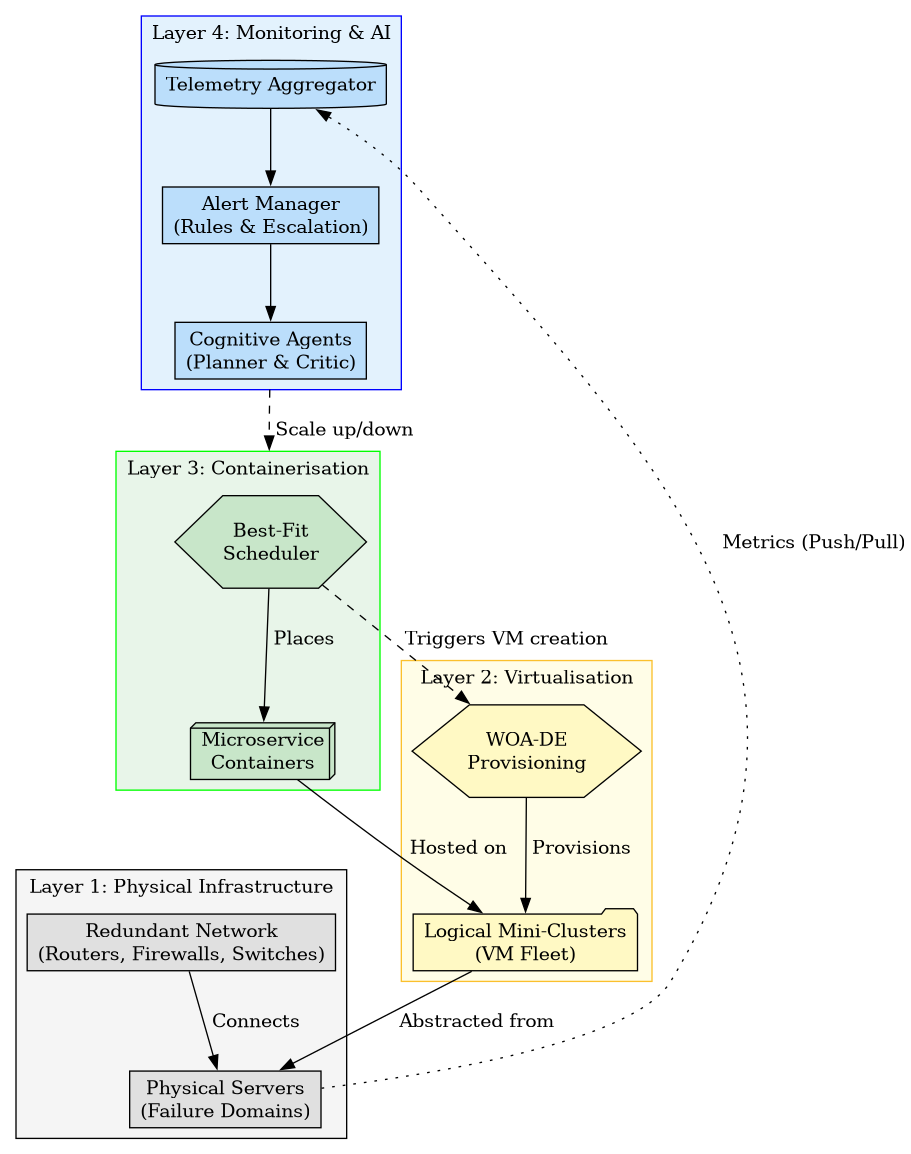
\includegraphics[width=0.95\linewidth, keepaspectratio]{cluster_full.gv.png}
\caption{The hierarchical four-layer architecture of the cluster ecosystem, showing
the data flow from physical infrastructure to the monitoring intelligence stratum.}
\label{fig:cluster_full}
\end{figure}

% ─────────────────────────────────────────────────────────────────
\section{Physical and Network Foundation}

\subsection{Physical Infrastructure and Failure Domains}

The physical layer comprises a fleet of servers interconnected by a managed switching
fabric that enforces bounded latency for intra-cluster communication. At the cluster
perimeter, stateful packet inspection filters unauthorised ingress traffic before it
reaches any internal resource. Core routing equipment manages inter-segment traffic
and public internet connectivity.

To satisfy availability constraints, the physical layer is designed around explicit
\textit{failure domains}. A failure domain is defined as a group of servers sharing
a common point of vulnerability --- a shared power distribution unit, a single
top-of-rack switch, or a single physical host. Higher-level scheduling algorithms
are programmed to distribute workload replicas across distinct failure domains;
a hardware event affecting one domain therefore cannot eliminate all instances of a
given service. All core routing and switching equipment is deployed in high-availability
pairs to eliminate network-partitioning risk, as illustrated in
Figure~\ref{fig:layer1_physical}.

\begin{figure}[htbp]
\centering
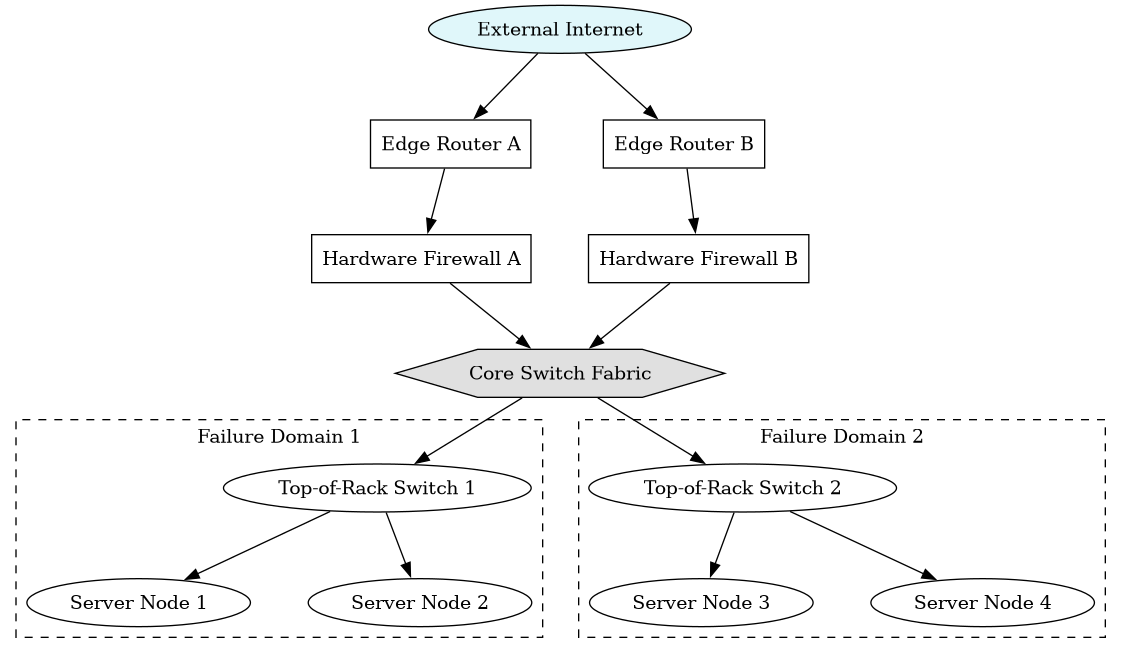
\includegraphics[width=0.85\linewidth, keepaspectratio]{layer1_physical.gv.png}
\caption{Physical infrastructure layer: explicit failure domains and redundant
switching fabric design.}
\label{fig:layer1_physical}
\end{figure}

\subsection{Overlay Network Architecture}

Physical compute abstraction is insufficient for multi-tenant security without an
equivalent abstraction at the network layer. An overlay network decouples the
logical topology from the physical cabling, permitting dynamic segmentation without
hardware reconfiguration.

\paragraph{Three-segment isolation model.}
The overlay network is partitioned into exactly three logical segments, corresponding
to the three distinct trust domains present in the target deployment. The first
segment hosts the workloads of tenant group A. The second hosts tenant group B. The
third is reserved for the observability and monitoring infrastructure.

Three segments, rather than two or four, follow directly from the threat model.
Merging the two tenant groups into a single segment would allow a compromised service
in one group to reach services in the other without crossing a firewall boundary ---
unacceptable when the two groups operate under different administrative and
organisational domains. Merging the monitoring segment into a tenant segment would
expose telemetry data to tenant traffic and risk losing observability during a
tenant-side incident. Subdividing beyond three would not add a distinct trust boundary;
it would only add routing complexity. Three segments is therefore the minimal
partitioning that satisfies the isolation requirement \cite{saxena2022secure}.

\paragraph{Routing and access control.}
All inter-segment traffic passes through a central, software-defined virtual router
operating under a \textit{default-deny} posture: any packet not matched by an
explicit permit rule is silently discarded. Cross-segment communication requires
bidirectional policy rules. The monitoring segment may initiate data collection
connections into the tenant segments; no connection originating from a tenant segment
toward the monitoring infrastructure is permitted. Outbound internet access is
provided via network address translation, masking the internal cluster topology from
external networks.

\begin{figure}[htbp]
\centering
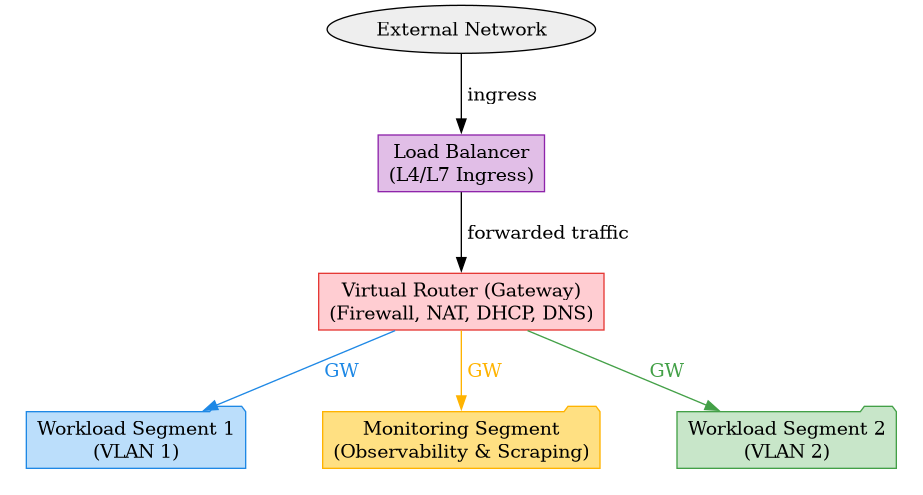
\includegraphics[width=0.8\linewidth, keepaspectratio]{virtual_network.gv.png}
\caption{Overlay network topology: a central virtual router enforces default-deny
policies and isolates the three logical segments by distinct trust level.}
\label{fig:vnet}
\end{figure}

% ─────────────────────────────────────────────────────────────────
\section{Virtualisation and VM Placement}

\subsection{Mini-Cluster Partitioning}

The VM fleet is partitioned into $k$ logical \textit{mini-clusters}, where each
mini-cluster groups VMs that host containers with strong mutual communication. The
rationale for this decomposition is threefold.

\textbf{Scheduling complexity.} Without partitioning, the placement algorithm
evaluates $n$ physical machines for every VM request. With $k$ mini-clusters of
roughly equal size, the search space per invocation shrinks to approximately
$\lfloor n/k \rfloor$ machines, reducing scheduling latency proportionally. For
on-line provisioning --- where placement decisions are made under live traffic --- this
reduction is operationally significant \cite{alahmad2024multiple}.

\textbf{Equitable resource distribution.} Partitioning prevents a subset of
high-demand VMs from monopolising the physical hosts nearest to the orchestration
plane. Each mini-cluster attracts a bounded subset of the workload, distributing
resource pressure across the full physical fleet.

\textbf{Behavioural homogeneity.} VMs within the same mini-cluster host services
with similar access patterns and scaling behaviour. This homogeneity means that a
scaling decision --- adding RAM, for instance --- generalises across the mini-cluster:
the same physical target serves any VM in the group. This property becomes
increasingly valuable as the number of VMs grows and individual case-by-case analysis
becomes infeasible.

A cross-boundary VM --- one whose container must communicate heavily with containers
in a different mini-cluster --- represents a partitioning error. In the static
assignment strategy, this is prevented at design time by mapping the mini-cluster
boundaries to the application's dependency graph; services with strong mutual
affinity are grouped into the same mini-cluster before any VM is provisioned. A
mispartitioned VM increases inter-segment network traffic, degrades placement
algorithm efficiency (the most suitable host may lie outside the search space), and
undermines the homogeneity property. Detection of systematic cross-boundary traffic
is one of the triggers for dynamic repartitioning in the long-term evolution of the
system.

\textbf{Determining $k$.} Two strategies govern the choice of $k$
\cite{tuli2023cilp, saxena2022proactive}. In the \textbf{static} approach, $k$ is
fixed from the application's architectural dependency graph at design time; services
sharing data paths are co-located in the same cluster. In the \textbf{dynamic}
approach, a machine learning model continuously analyses inter-VM communication
matrices and resource correlation patterns, adjusting cluster boundaries as the
application evolves. The present implementation uses the static strategy; the dynamic
approach is identified as a direction for future development.

\subsection{The Hybrid WOA-DE Placement Algorithm}

The VM provisioning algorithm addresses the following optimisation problem: given
a request for a new virtual machine with a specified resource requirement vector,
which physical machine within the target mini-cluster should host it? A hybrid
algorithm integrating the \textbf{Whale Optimisation Algorithm} (WOA)
\cite{mirjalili2016woa} and \textbf{Differential Evolution} (DE) \cite{storn1997de}
is adopted. The application of evolutionary strategies to VM allocation is well
established in the literature \cite{zhang2020intelligent}, and WOA has demonstrated
particular efficacy in multi-objective placement settings \cite{saxena2022secure}.

\paragraph{Design rationale.}
WOA mathematically models the bubble-net hunting behaviour of humpback whales.
Candidate solutions are updated by either contracting towards the best-known mapping
(exploitation) or spiralling around it (local intensification). DE generates trial
solutions via algebraic mutation and crossover of population members, providing
superior spatial exploration. Pure WOA is vulnerable to premature convergence on
local optima. The hybrid design mitigates this by splitting the candidate population
at each iteration: one subset undergoes WOA position updates (deep exploitation)
while the other undergoes DE mutation (diversity maintenance). This combination
prevents stagnation while guaranteeing monotonic population improvement.

\paragraph{Input and output.}
The algorithm receives a resource request vector comprising the required virtual
CPUs, memory, storage, and the target mini-cluster identifier, as well as a snapshot
of current host metrics drawn from the monitoring layer. It outputs the recommended
VM-to-host mapping and its associated fitness score.

\paragraph{Formal description.}
Let $n$ denote the population size and $T$ the maximum number of iterations. Each
candidate solution $X_i$ represents a complete mapping of virtual machines to
physical hosts within the selected mini-cluster. The quality of a mapping is
evaluated by the fitness function defined in Section~\ref{sec:fitness}.

Algorithm~\ref{alg:woade} presents the complete procedure.

\begin{algorithm}[htbp]
\DontPrintSemicolon
\SetKwInOut{KwIn}{Input}
\SetKwInOut{KwOut}{Output}
\SetKw{KwAnd}{and}
\SetKw{KwOr}{or}
\SetKw{KwInit}{Initialise}

\KwIn{Resource request vector $(v_{\text{cpu}}, v_{\text{ram}}, v_{\text{io}})$;
      target mini-cluster $\mathcal{C}$; host metric snapshot $\mathcal{M}$;
      population size $n$; max iterations $T$;
      WOA spiral constant $b$; DE scale factor $F$; DE crossover rate $CR \in (0,1)$}
\KwOut{Optimal VM-to-host mapping $X^*$; fitness score $f(X^*)$}

\BlankLine
\tcp{Phase 1 — Initialisation}
Randomly generate $n$ candidate mappings $\{X_0, X_1, \ldots, X_{n-1}\}$ within feasible placement bounds derived from $\mathcal{C}$ and $\mathcal{M}$\;
Evaluate $f(X_i)$ for all $i$\;
$X^* \leftarrow \arg\min_i f(X_i)$\;
Set $a_0 \leftarrow 2$\;

\BlankLine
\tcp{Phase 2 — Main evolutionary loop}
\For{$t \leftarrow 0$ \KwTo $T$}{
    Compute $a \leftarrow 2\!\left(1 - t/T\right)$\;
    Draw $r_1, r_2 \sim \mathrm{Uniform}(0,1)$\;
    Compute $A \leftarrow 2a\,r_1 - a$ \KwAnd $C \leftarrow 2\,r_2$\;
    
    \BlankLine
    \tcp{WOA update sub-phase (first half of population)}
    \ForEach{$X_i$ in WOA subset}{
        Draw $p \sim \mathrm{Uniform}(0,1)$\;
        \eIf{$p < 0.5$}{
            \eIf{$|A| < 1$ \upshape{(exploitation)}}{
                $D \leftarrow |C \cdot X^* - X_i(t)|$\;
                $X_i(t{+}1) \leftarrow X^* - A \cdot D$\;
            }{
                Select $X_\mathrm{rand}$ uniformly from population\;
                $D \leftarrow |C \cdot X_\mathrm{rand} - X_i(t)|$\;
                $X_i(t{+}1) \leftarrow X_\mathrm{rand} - A \cdot D$\;
            }
        }{
            \tcp{Spiral bubble-net update}
            $D \leftarrow |X^* - X_i(t)|$\;
            Draw $l \sim \mathrm{Uniform}(-1,1)$\;
            $X_i(t{+}1) \leftarrow D\,e^{bl}\cos(2\pi l) + X^*(t)$\;
        }
        Update $X^*$ if $f(X_i(t{+}1)) < f(X^*)$\;
    }
    
    \BlankLine
    \tcp{DE mutation–crossover–selection sub-phase (second half)}
    \ForEach{$X_j$ in DE subset}{
        Select distinct $X_{r_1}, X_{r_2}$ from population\;
        $V_j \leftarrow X^* + F \cdot (X_{r_1} - X_{r_2})$ \tcp*{mutation}
        \ForEach{component $k$}{
            \eIf{$\mathrm{rand}() \leq CR$}{
                $U_j[k] \leftarrow V_j[k]$\;
            }{
                $U_j[k] \leftarrow X_j[k]$\;
            }
        }
        \If{$f(U_j) < f(X_j)$}{$X_j \leftarrow U_j$} \tcp*{greedy selection}
        Update $X^*$ if $f(X_j) < f(X^*)$\;
    }
}

\BlankLine
\Return $X^*$, $f(X^*)$\;
\caption{Hybrid WOA-DE VM Placement Algorithm}
\label{alg:woade}
\end{algorithm}

\begin{figure}[htbp]
\centering
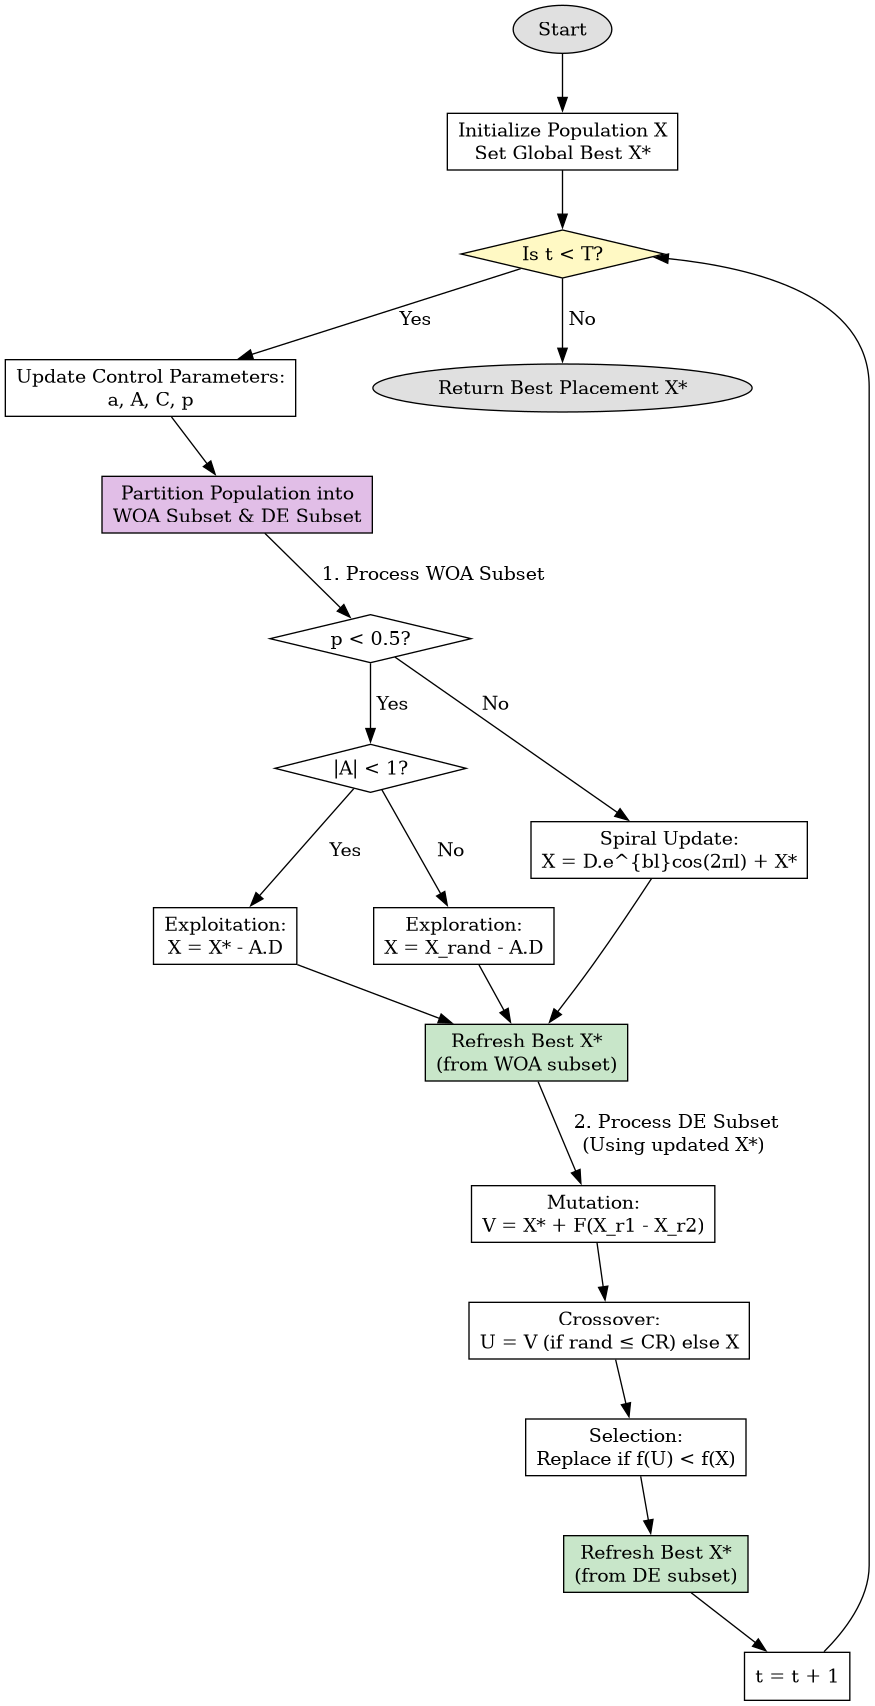
\includegraphics[width=0.88\linewidth, height=0.8\textheight, keepaspectratio]{flowchart.gv.png}
\caption{Flowchart of the hybrid WOA-DE provisioning algorithm, highlighting the parallel
WOA and DE evaluation phases and the convergence condition.}
\label{fig:flowchart}
\end{figure}

\paragraph{Algorithmic properties.}
The dual exploration mechanics --- WOA's distance-based spiral geometry and DE's
algebraic mutation --- jointly suppress local optima stagnation. The DE greedy
selection phase guarantees monotonic population improvement, ensuring algorithmic
convergence. Because both algorithms evaluate fitness analytically, they accommodate
the discretisation required to map continuous numerical outputs back to feasible,
discrete host assignments.

\subsection{Fitness Function}
\label{sec:fitness}

Each candidate placement is evaluated by a fitness function that acts on four
resource dimensions: CPU capacity ($C$), RAM ($R$), I/O throughput ($IO$), and
energy consumption ($E$). The function must satisfy two design requirements that
pull in opposite directions: it must treat all four dimensions equitably regardless
of their physical units, and it must penalise near-exhaustion more aggressively than
slight under-utilisation.

\paragraph{Normalisation.}
The four metrics occupy incompatible numerical scales. RAM is measured in gigabytes;
energy is measured in joules per hour; a raw difference of 1 GB in memory and 1 J
in energy are not comparable without rescaling. Each metric is normalised to a
Z-score prior to evaluation:

\[
  X_i^* = \frac{X_i - \bar{X}}{\sigma_X}
\]

where $\bar{X}$ is the mean and $\sigma_X$ the standard deviation computed across
all candidate hosts in the mini-cluster at the time of the placement request. After
normalisation, a unit deviation in CPU usage and a unit deviation in energy
consumption carry equal weight in the fitness computation.

\paragraph{Weighted Euclidean distance.}
The aggregate score is computed as a weighted Euclidean distance over the four
normalised resource gaps:

\[
  \text{fitness} =
    \sqrt{w_1 \cdot (\Delta C)^2 + w_2 \cdot (\Delta R)^2
        + w_3 \cdot (\Delta IO)^2 + w_4 \cdot (\Delta E)^2}
\]

where $\Delta X$ is the difference between the resource quantity requested by the
incoming VM and the quantity available on the candidate host. Squaring the gaps
serves a specific purpose: a host with 5\% remaining CPU headroom receives a penalty
that is an order of magnitude larger than one with 50\% remaining, even if the
absolute difference in the $\Delta C$ terms is modest. This non-linear penalisation
is the mechanism by which the fitness function prioritises availability over
aggregate utilisation.

\paragraph{Weight vector and default values.}
The weights $(w_1, w_2, w_3, w_4)$ are real-valued parameters summing to unity:

\[
  \sum_{i=1}^{4} w_i = 1, \quad w_i \geq 0.
\]

At initialisation, the weight vector is set to the uniform prior
$w_i = 0.25\ \forall i$, expressing no prior knowledge about which resource
dimension is the binding constraint. This baseline is chosen for its reproducibility:
any deployment starts from the same configuration regardless of hardware
heterogeneity. The weight vector is subsequently adjusted by the predictive model
described in Section~\ref{sec:prediction}; if the cluster enters a phase of sustained
RAM pressure, $w_2$ increases and the remaining weights decrease proportionally,
causing the algorithm to prioritise memory-rich hosts in subsequent placements. The
application designer may also override the initial vector to encode domain knowledge
--- for example, setting a higher $w_4$ for deployments where energy cost is a
primary concern.

The algorithm seeks to \textit{minimise} this score; the placement recommended is
that which leaves the host with the largest, most balanced resource surplus across
all four dimensions.

\subsection{Reactive Scaling}

Two complementary scaling modes are triggered by monitoring-layer alerts:

\textbf{Horizontal scaling} addresses scenarios in which request volumes exceed the
processing capacity of the current workload instances. It is triggered when HTTP 5xx
error rates surpass defined thresholds (1\% at warning severity, 5\% at critical
severity), or when network packet loss exceeds 2\%. The response involves instantiating
a new, identical host. The WOA-DE algorithm determines its optimal physical placement,
and the new instance is appended to the load-balancing pool to immediately absorb
excess traffic \cite{sung2024cloning}.

\textbf{Vertical scaling} targets resource saturation intrinsic to a specific host.
CPU utilisation exceeding 80\% (warning) or 95\% (critical) triggers the allocation
of an additional virtual core. Memory utilisation exceeding 80\% triggers a 20\%
capacity increase. When the current physical host lacks sufficient free capacity for
vertical expansion, the orchestration layer initiates a live migration: the WOA-DE
algorithm is invoked to identify an optimal destination host, and the workload is
relocated without interruption \cite{lai2025energy}.

Table~\ref{tab:thresholds} summarises the complete threshold matrix.

\begin{table}[htbp]
\centering
\caption{Reactive scaling threshold matrix.}
\label{tab:thresholds}
\begin{tabular}{L{3cm} C{2cm} C{2cm} L{4.5cm}}
\toprule
\textbf{Metric} & \textbf{Warning (\%)} & \textbf{Critical (\%)} & \textbf{Remediation} \\
\midrule
CPU utilisation         & 80  & 95  & Add 1 virtual core; migrate if host saturated \\
RAM utilisation         & 60  & 80  & Add 20\% RAM; migrate if host saturated \\
Disk I/O free           & $<$20 & $<$10 & Add 15 GB disk; migrate if host saturated \\
HTTP 5xx error rate     & 1   & 5   & Horizontal scaling (new instance) \\
Network packet loss     & ---  & 2   & Horizontal scaling (new instance) \\
\bottomrule
\end{tabular}
\end{table}

% ─────────────────────────────────────────────────────────────────
\section{Containerisation and Workload Scheduling}

The containerisation layer manages the execution of application workloads across the
virtual machine fleet. While the WOA-DE hybrid algorithm governs the mapping of
virtual machines to physical hardware, workload-to-VM scheduling employs a deliberate
\textbf{Best-Fit} heuristic. For each pending workload unit, the scheduler identifies
the active virtual machine that possesses the minimum available capacity sufficient to
satisfy the workload's resource request.

Best-Fit minimises resource fragmentation across the VM fleet
\cite{begam2020timer}. By packing active virtual machines to near-maximum capacity,
it maximises the fraction of VMs that are entirely idle. Idle instances can then be
suspended or powered down, yielding reductions in energy consumption and licensing
overhead \cite{yang2025task}. The scheduler additionally applies affinity rules: workload
units belonging to the same service group are preferentially placed within their
designated mini-cluster, preserving network locality and limiting cross-boundary
traffic.

% ─────────────────────────────────────────────────────────────────
\section{Monitoring and Observability Architecture}

\subsection{Telemetry Collection}

The monitoring subsystem employs a pull-based collection architecture: a central
aggregation component periodically requests metric samples from agents deployed on
every managed node \cite{nguyen2022load}. The collection scope spans all four layers:
physical server metrics (thermal, power, storage I/O, conforming to data-centre
infrastructure monitoring standards \cite{balabanov2025dcim}), hypervisor metrics such as
CPU steal time and memory balloon activity, software-defined network throughput, and
application-layer health endpoints.

Collected telemetry is subjected to time-windowed retention policies. High-resolution
data is preserved during anomalous events; normal baseline periods are subject to
progressive downsampling to bound storage growth \cite{bompotas2025commc}.

\subsection{Alert Management}

The alert management subsystem translates raw metric time-series into actionable
orchestration commands. When a metric breaches a defined threshold, the subsystem
emits a structured alert payload. To prevent \textit{alert storms} --- conditions
in which a single physical failure triggers thousands of downstream alerts across
dependent workloads --- the subsystem implements grouping and inhibition rules
\cite{gu2023towards}. Related symptoms are consolidated into a single root-cause alert;
only that consolidated alert is forwarded to the orchestration engine.

Table~\ref{tab:metric_categories} classifies the principal categories of monitored
metrics and their architectural purpose.

\begin{table}[htbp]
\centering
\caption{Monitored metric categories and their observability purposes.}
\label{tab:metric_categories}
\begin{tabular}{L{3.5cm} L{3.5cm} L{6cm}}
\toprule
\textbf{Category} & \textbf{Sources} & \textbf{Purpose} \\
\midrule
Hardware health     & Physical hosts, power units     & Detect hardware degradation; inform failure-domain isolation \\
CPU utilisation     & All virtual hosts               & Trigger vertical scaling and live migration \\
Memory utilisation  & All virtual hosts               & Trigger RAM expansion or migration \\
Disk I/O throughput & All virtual hosts               & Detect I/O saturation; trigger disk expansion \\
Network throughput  & Overlay network devices         & Monitor inter-segment traffic; detect anomalous flows \\
Application errors  & Workload health endpoints       & Trigger horizontal scaling on elevated 5xx rates \\
Energy consumption  & Physical hosts, workload agents & Inform energy-weighted placement decisions \\
Workload availability & Uptime probes               & Detect unreachable instances; trigger failover \\
\bottomrule
\end{tabular}
\end{table}

% ─────────────────────────────────────────────────────────────────
\section{Intelligence and Security}

\subsection{Predictive Model and Dynamic Weight Recalibration}
\label{sec:prediction}

Fixed alert thresholds assume that the workload distribution on the cluster is
stationary, an assumption that fails for microservices deployments subject to
diurnal traffic cycles and application version changes. A gradient-boosted predictive
model replaces this rigidity: it analyses the current metric snapshot across all
monitored VMs and outputs both a bottleneck classification and a recalibrated weight
vector for the placement fitness function.

The model's primary output is a revised $(w_1, w_2, w_3, w_4)$ vector. If the
cluster exhibits sustained RAM pressure --- a bottleneck that pure threshold logic
may not detect until multiple VMs cross their warning levels simultaneously ---
the model increases $w_2$ and reduces the others proportionally, shifting the
placement algorithm's priorities before the next VM request arrives. Similarly,
a period of elevated energy consumption pushes $w_4$ upward, directing the algorithm
toward energy-efficient hosts.

The model also predicts dynamic alert thresholds for CPU, RAM, and HTTP error rates.
These replace the static percentage values in Table~\ref{tab:thresholds} with
context-sensitive values calibrated to the current baseline behaviour of the fleet.

\textbf{Limitation on incremental learning.} The predictive model is not natively
trained in an online manner. Gradient-boosted tree models do not support parameter-level
updates from individual observations the way neural networks do; online learning
requires either appending new trees to the existing ensemble or retraining from a
growing dataset. The current architecture uses batch re-inference with
soft-label pseudo-targets derived from the model's own previous predictions to
approximate adaptation. This approach carries a known risk of model collapse under
distribution shift: if the pseudo-labels diverge from the true cluster state, the
model may reinforce its own errors over successive batches. Ground-truth labels for
supervised retraining --- derived from post-hoc resolution outcomes of detected
alerts --- have not yet been collected; the incremental update mechanism is therefore
disabled in the present implementation and is identified as a required engineering
step before production deployment.

\subsection{Dual-Agent Decision System}

Safe autonomous remediation requires a separation between the agent that proposes
actions and the agent that authorises them. A single agent combining both functions
can rationalise unsafe actions to itself; an independent validator with no investment
in the proposal cannot.

The \textbf{Planner} observes the cluster state by executing a mandatory sequence of
read operations --- health summary, bottleneck prediction, recent action log, warning
queue, node statistics, targeted resource detail --- before formulating a remediation
proposal. The proposal is expressed as a structured record containing the intended
tool, its parameters, the initiating risk class, an expected effect, and a rollback
procedure. The Planner does not execute any write operation.

The \textbf{Critic} receives the proposal and the current cluster snapshot and
evaluates it against a formal constraint set. Table~\ref{tab:critic_constraints}
specifies the seven constraints, the trigger condition for each, the verdict issued
when violated, and the alternative action suggested.

\begin{table}[htbp]
\centering
\caption{Formal Critic constraint set.}
\label{tab:critic_constraints}
\begin{tabular}{C{0.4cm} L{3.2cm} L{3.8cm} L{3.2cm} L{2.6cm}}
\toprule
\textbf{\#} & \textbf{Constraint} & \textbf{Trigger condition} & \textbf{Verdict} & \textbf{Alternative} \\
\midrule
1 & Node headroom (CPU)
  & Target host CPU $> 85\%$ at time of evaluation
  & REJECT
  & \texttt{migrate\_vm} to a host with CPU $< 80\%$ \\
\addlinespace
2 & Node headroom (RAM)
  & Target host RAM $> 85\%$
  & REJECT
  & Clone instance; migrate if no eligible host \\
\addlinespace
3 & Cluster saturation
  & No host has CPU $< 80\%$
  & REJECT scale-up actions
  & Delete or suspend idle instances first \\
\addlinespace
4 & Duplicate action
  & Identical (tool, resource ID) pair in the action log within the last 5 minutes
  & REJECT
  & Wait for previous action to stabilise \\
\addlinespace
5 & Execution loop
  & Same (tool, resource ID) pair executed 3 or more times in 24 hours without resolution
  & REJECT; escalate to HIGH risk
  & Propose a fundamentally different remediation \\
\addlinespace
6 & Direction correctness
  & Scale-down proposal specifies equal or greater resource than current; scale-up specifies equal or fewer replicas
  & REJECT
  & Correct the direction; re-propose \\
\addlinespace
7 & Bottleneck alignment
  & Proposed action targets a resource dimension orthogonal to the detected bottleneck
  & FLAG (not reject); require explicit justification in reason field
  & Propose a resource-aligned action \\
\bottomrule
\end{tabular}
\end{table}

The Critic operates under a \textit{monotonic risk policy}: the risk classification
of a proposal may be escalated but never reduced. Enforcement is structural:
the final risk level is computed as the maximum of the static floor defined by the
action type, the Planner's declared level, and the Critic's assessment. An adversarial
prompt that attempts to reclassify a destructive action as low-risk is therefore
defeated by the static floor, regardless of the reasoning presented.

\begin{figure}[htbp]
\centering
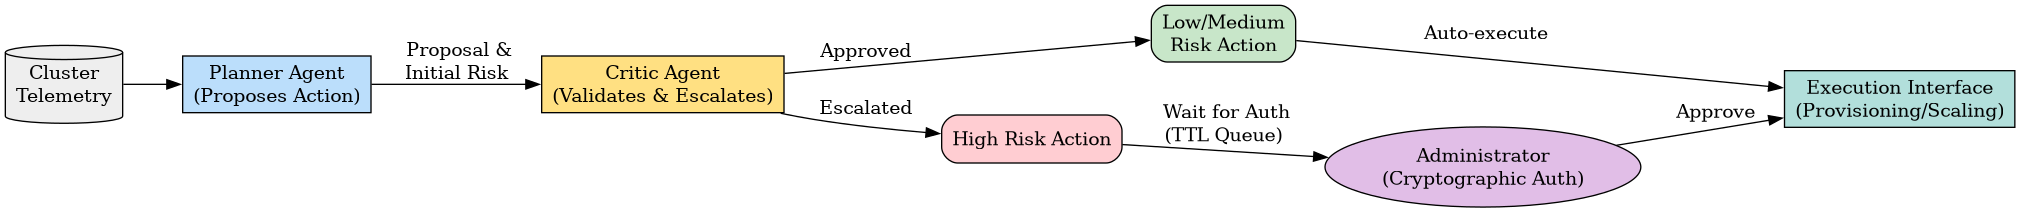
\includegraphics[width=\linewidth, keepaspectratio]{ai_security.gv.png}
\caption{Dual-agent decision system: the Planner proposes, the Critic validates
against the formal constraint set, and the execution layer acts only on approved
proposals.}
\label{fig:ai_security}
\end{figure}

\subsection{Risk-Based Escalation Matrix}

The execution authority of the agent system is strictly governed by a three-tier
escalation matrix, presented in Table~\ref{tab:risk_matrix}.

\begin{table}[htbp]
\centering
\caption{Risk-based escalation matrix for autonomous action execution.}
\label{tab:risk_matrix}
\begin{tabular}{C{2cm} L{4.5cm} L{4.5cm} C{2cm}}
\toprule
\textbf{Risk tier} & \textbf{Action types} & \textbf{Execution policy} & \textbf{Human required} \\
\midrule
Low
  & Add virtual CPUs, increase deployment replicas
  & Executed autonomously upon Critic approval; logged immediately
  & No \\
\addlinespace
Medium
  & Reduce virtual resources, live migration, container restart, clone instance \cite{sung2024cloning}
  & Executed autonomously upon Critic approval; operator notified by log
  & No \\
\addlinespace
High
  & Power off workload, delete instance, delete deployment, drain physical node
  & Halted; queued in approval log; administrator notified; executed only upon explicit authorisation
  & Yes \\
\bottomrule
\end{tabular}
\end{table}

\subsection{Security Architecture}

The integration of autonomous cognitive agents into an infrastructure management
pipeline creates attack surfaces that are absent from manually administered clusters.
An agent that can execute VM migrations, scale deployments, and stop running services
is a powerful target: a successful adversarial injection into its reasoning context
could cause it to misclassify a destructive action as routine, to disable monitoring,
or to drain a critical node under load. The security model is therefore structured
around the specific threats introduced by the agent architecture, not around a generic
checklist of security properties.

\paragraph{Threat: lateral movement from a compromised tenant workload.}
The three-segment overlay network with default-deny routing prevents a compromised
container in the hospital or ministry segment from reaching the monitoring
infrastructure or the orchestration API. A container that establishes an unexpected
outbound connection hits the implicit deny rule before its packets reach the
monitoring segment. The monitoring plane is thus reachable from the outside only
through explicit permit rules, which are limited to the telemetry collection protocol.

\paragraph{Threat: forged remediation commands.}
All internal API calls within the orchestration pipeline require a shared API key
validated at every endpoint. A forged proposal injected at any stage is rejected
before execution. Telemetry collection traffic and command traffic are transmitted
over encrypted channels, preventing passive observation of API key material by
an attacker with access to the physical network.

\paragraph{Threat: adversarial prompt injection into agent reasoning.}
If a malicious actor embeds instructions inside a VM's hostname, metric labels, or
log output that the Planner reads during its mandatory data collection sequence, those
instructions could influence the proposed action. Two mechanisms limit this risk.
First, the Critic evaluates the proposal independently against the formal constraint
table (Table~\ref{tab:critic_constraints}); an injected instruction that leads the
Planner to propose an unsafe action is caught by Constraint~1--7 before execution.
Second, the monotonic risk floor prevents the injected content from lowering the risk
classification of a destructive action below its static type-level floor.

\paragraph{Threat: privilege escalation through the agent's execution scope.}
The Planner and Critic agents hold no infrastructure credentials. They output
structured proposals to a separate execution layer, which performs secondary
validation and issues the actual API call. An agent that is manipulated to propose
an unusually broad action still cannot execute it without passing through the execution
layer's validation.

\paragraph{Audit and forensic traceability.}
Every proposal, Critic verdict, execution outcome, and human approval is appended
to an immutable log \cite{gu2023towards, saxena2022secure}. The append-only property
ensures that a compromised agent cannot remove evidence of actions it has taken.
Post-incident forensic analysis can therefore reconstruct the full decision chain
leading to any infrastructure change.

\paragraph{Workload hardening.}
Virtual machine images are built with minimal driver sets to reduce the kernel attack
surface. Container workloads run with a restricted capability set; persistent
write access to the filesystem is granted only where the application explicitly
requires it. Scheduling affinity rules separate workloads from different security
domains onto distinct physical hosts, limiting the blast radius of a kernel-level
side-channel attack \cite{saxena2022secure}.

% ─────────────────────────────────────────────────────────────────
\section{Conclusion}

The four design gaps identified at the close of Chapter~1 are each addressed by a
specific component of the architecture developed here. The WOA-DE hybrid algorithm
resolves the premature convergence problem of single-paradigm bio-inspired
optimisers through population splitting: one subset exploits the current best
placement via WOA's spiral geometry while the other maintains diversity through
DE's algebraic mutation. The multi-objective fitness function with Z-score
normalisation and quadratic penalisation integrates CPU, RAM, I/O, and energy into
a single comparable score, sidestepping the unit-incommensurability problem that
causes single-objective heuristics to produce systematically skewed placements.
The XGBoost prediction layer closes the loop between monitoring and placement by
recalibrating the fitness weight vector in response to observed bottleneck patterns,
replacing the static weight assignment that all prior work assumes. Finally, the
Planner/Critic system with its formal seven-constraint validation table and monotonic
risk floor provides autonomous remediation authority bounded by explicit, auditable
governance rules --- a requirement that the reviewed literature does not address.

What this chapter does not provide is an empirical evaluation of these mechanisms.
Performance claims --- that the WOA-DE hybrid converges faster than pure WOA on
a placement problem of a given dimension, or that the weight recalibration loop
reduces mean time to recovery --- remain to be measured. Chapter~3 describes the
implementation and identifies the experiments required.


% ============================================================
%  CHAPTER 3 — IMPLEMENTATION
% ============================================================
%% ---------------------------------------------------------------
%% TODO (student): Complete the following before final submission:
%%   - Replace all [PLACEHOLDER] figures with actual screenshots
%%   - Fill in the VM inventory table from Proxmox
%%   - Fill in the Kubernetes object table from kubectl output
%%   - Add performance measurement results if available
%% ---------------------------------------------------------------
\chapter{Implementation}

\section{Introduction}

Chapter~2 described what the infrastructure must do and why each design decision was
made. This chapter describes how those decisions were realised, which technologies
were selected, and what the resulting system looks like at the configuration level.
The exposition is grounded directly in the project artefacts: the source code, the
network router configuration, the monitoring rule files, and the service deployment
descriptors. Where these artefacts do not yet cover a section --- because the physical
deployment was not finalised at the time of writing --- the gap is marked explicitly
with~[TO BE CONFIRMED] and must be completed before submission.

% ─────────────────────────────────────────────────────────────────
\section{Technology Selection and Justification}

For each architectural layer defined in Chapter~2, a specific technology was selected
on the basis of licence model, community maturity, on-premises suitability, and
performance characteristics. Table~\ref{tab:tech_selection} summarises these choices.

\begin{table}[htbp]
\centering
\caption{Technology selection by architectural layer.}
\label{tab:tech_selection}
\begin{tabular}{L{3cm} L{2.8cm} C{1.8cm} L{5.5cm}}
\toprule
\textbf{Architectural layer} & \textbf{Technology} & \textbf{Version} & \textbf{Justification} \\
\midrule
Virtualisation         & Proxmox VE     & [TO BE CONFIRMED] & Open-source (AGPL), integrates KVM and LXC natively, REST API, HA and live migration without vendor cost \\
Container orchestration & Kubernetes    & [TO BE CONFIRMED] & CNCF-graduated; rich scheduler primitives, namespace isolation, HPA, NetworkPolicy; dominant community \\
Monitoring             & Prometheus     & [TO BE CONFIRMED] & Pull-based scraping, PromQL, HTTP SD; native Kubernetes integration; \textsc{CNCF} flagship project \\
Visualisation          & Grafana        & [TO BE CONFIRMED] & Open-source dashboarding; native Prometheus datasource; alerting integration \\
Virtual routing        & OPNsense       & [TO BE CONFIRMED] & Open-source BSD firewall; per-interface VLAN routing, stateful packet inspection, NAT, REST API \\
AI agent framework     & Agno (Python)  & [TO BE CONFIRMED] & Lightweight multi-agent library; tool-call abstraction; SQLite-backed agent memory \\
Prediction model       & XGBoost        & [TO BE CONFIRMED] & Gradient boosting; low inference latency; interpretable feature importances; established in cluster resource prediction literature; ensemble extension supports batch re-inference for weight recalibration \\
LLM inference          & Groq Cloud API & ---               & Sub-second LLM inference for Planner/Critic reasoning (llama-3.3-70b-versatile) \\
Service discovery API  & FastAPI (Python) & [TO BE CONFIRMED] & Asynchronous HTTP; Pydantic validation; native OpenAPI documentation \\
\bottomrule
\end{tabular}
\end{table}

% ─────────────────────────────────────────────────────────────────
\section{Implementation Environment}

The proof-of-concept cluster is deployed on-premises at the USTHB Faculty of
Informatics. It consists of physical servers connected via a managed switching
fabric, administered through the Proxmox VE hypervisor management interface.

\begin{table}[htbp]
\centering
\caption{Physical host inventory. All values are to be confirmed from the Proxmox
\texttt{Datacenter} view.}
\label{tab:host_inventory}
\begin{tabular}{C{1.8cm} L{2.5cm} C{2cm} C{2cm} C{2.2cm} C{2.2cm}}
\toprule
\textbf{Host ID} & \textbf{Role} & \textbf{CPU} & \textbf{RAM} & \textbf{Storage} & \textbf{OS} \\
\midrule
pfe0 & [TO BE CONFIRMED] & [TBC] & [TBC] & [TBC] & [TBC] \\
pfe1 & [TO BE CONFIRMED] & [TBC] & [TBC] & [TBC] & [TBC] \\
pfe2 & [TO BE CONFIRMED] & [TBC] & [TBC] & [TBC] & [TBC] \\
pfe3 & [TO BE CONFIRMED] & [TBC] & [TBC] & [TBC] & [TBC] \\
pfe4 & [TO BE CONFIRMED] & [TBC] & [TBC] & [TBC] & [TBC] \\
pfe5 & [TO BE CONFIRMED] & [TBC] & [TBC] & [TBC] & [TBC] \\
pfe6 & [TO BE CONFIRMED] & [TBC] & [TBC] & [TBC] & [TBC] \\
pfe7 & [TO BE CONFIRMED] & [TBC] & [TBC] & [TBC] & [TBC] \\
\bottomrule
\end{tabular}
\end{table}

The cluster encompasses eight physical nodes, identified as \texttt{pfe0} through
\texttt{pfe7}. Nodes are partitioned into two primary roles: Kubernetes worker nodes
hosting application and monitoring workloads, and dedicated Kubernetes master nodes
forming the control plane. A subset of nodes additionally hosts LXC containers for
lightweight infrastructure services. Detailed CPU, RAM, and storage specifications
are to be confirmed from the Proxmox Datacenter inventory following finalisation of
the hardware allocation.

\begin{figure}[htbp]
\centering
\fbox{\rule{0pt}{5cm}\rule{0.9\linewidth}{0pt}}
\caption{[PLACEHOLDER --- Screenshot of: Proxmox VE Datacenter node summary view,
listing pfe0 through pfe7 with CPU and memory utilisation bars.]}
\label{fig:placeholder_pve_nodes}
\end{figure}

% ─────────────────────────────────────────────────────────────────
\section{Virtualisation with Proxmox VE}

Proxmox VE implements the virtualisation layer defined in Chapter~2, providing KVM-based
virtual machine management and LXC container support through a unified web interface
and REST API. The platform supports live migration between cluster nodes, shared storage
pools, and high-availability VM groups, directly instantiating the failure-domain
redundancy model described in Section~2.4.

Virtual machines are created via the Proxmox API or web interface with explicit
resource envelopes (vCPU count, RAM, disk size). Resource pools group VMs by
functional domain, and HA groups ensure that critical VMs are automatically restarted
on surviving nodes following a host failure. The WOA-DE placement algorithm
interfaces with the Proxmox REST API to query real-time node utilisation metrics and
to submit live migration commands when the fitness function determines that relocation
is warranted.

\begin{table}[htbp]
\centering
\caption{VM inventory. All values to be confirmed from the Proxmox
\texttt{pvenode list --full} output.}
\label{tab:vm_inventory}
\begin{tabular}{L{2.8cm} C{1.5cm} C{1.8cm} C{1.8cm} L{2.5cm} C{2cm}}
\toprule
\textbf{VM Name} & \textbf{vCPU} & \textbf{RAM} & \textbf{Disk} & \textbf{Hosted service} & \textbf{Mini-cluster} \\
\midrule
[TO BE CONFIRMED] & [TBC] & [TBC] & [TBC] & [TBC] & [TBC] \\
\multicolumn{6}{l}{\footnotesize\textit{(Repeat rows from Proxmox VM list)}} \\
\bottomrule
\end{tabular}
\end{table}

\begin{figure}[htbp]
\centering
\fbox{\rule{0pt}{5cm}\rule{0.9\linewidth}{0pt}}
\caption{[PLACEHOLDER --- Screenshot of: Proxmox VE web dashboard displaying the
VM summary table for the cluster with resource allocation and node placement.]}
\label{fig:placeholder_pve_dashboard}
\end{figure}

% ─────────────────────────────────────────────────────────────────
\section{Container Orchestration with Kubernetes}

Kubernetes implements the containerisation layer from Chapter~2. Each architectural
concept from that layer maps to a specific Kubernetes primitive:

The mini-cluster partitioning concept corresponds to Kubernetes \textbf{Namespaces}.
Each mini-cluster is realised as a distinct namespace, providing logical isolation,
independent resource quotas, and a scope for NetworkPolicy enforcement. Table~\ref{tab:k8s_objects}
lists the five namespaces instantiated for the proof-of-concept deployment.

Container scheduling within a mini-cluster corresponds to the \textbf{Kubernetes
Scheduler} operating under Pod resource requests and limits. The Best-Fit heuristic
is approximated by setting appropriate resource requests so the scheduler assigns
Pods to the most-occupied feasible node.

Horizontal scaling corresponds to \textbf{HorizontalPodAutoscaler} objects, which
increase replica counts when CPU or custom metrics exceed defined targets.

Service discovery corresponds to Kubernetes \textbf{Services} with cluster-internal
DNS resolution, allowing each microservice to reference its dependencies by name
rather than by IP address.

\begin{table}[htbp]
\centering
\caption{Kubernetes object inventory (partial --- to be completed with
\texttt{kubectl get all --all-namespaces} output).}
\label{tab:k8s_objects}
\begin{tabular}{L{2cm} L{3.5cm} L{3cm} L{5cm}}
\toprule
\textbf{Kind} & \textbf{Name} & \textbf{Namespace} & \textbf{Purpose} \\
\midrule
Namespace & mini-cluster-1 & --- & Authentication, blockchain, crypto, messaging \\
Namespace & mini-cluster-2 & --- & Clinical care services (hospital) \\
Namespace & mini-cluster-3 & --- & Hospital and patient management \\
Namespace & mini-cluster-4 & --- & Ministry-tier services and frontend \\
Namespace & mini-cluster-5 & --- & Facility management and hospital frontend \\
Deployment & auth & mini-cluster-1 & [TO BE CONFIRMED] \\
Deployment & blockchain-service & mini-cluster-1 & [TO BE CONFIRMED] \\
Deployment & cpabe-service & mini-cluster-1 & [TO BE CONFIRMED] \\
Deployment & rabbitmq & mini-cluster-1 & Asynchronous message broker \\
Deployment & soins & mini-cluster-2 & [TO BE CONFIRMED] \\
Deployment & rendez-vous & mini-cluster-2 & [TO BE CONFIRMED] \\
Deployment & consultations & mini-cluster-2 & [TO BE CONFIRMED] \\
Deployment & prescriptions-bilans-radios & mini-cluster-2 & [TO BE CONFIRMED] \\
Deployment & interventions & mini-cluster-2 & [TO BE CONFIRMED] \\
Deployment & hopitaux & mini-cluster-3 & [TO BE CONFIRMED] \\
Deployment & hospitalisations & mini-cluster-3 & [TO BE CONFIRMED] \\
Deployment & patients & mini-cluster-3 & [TO BE CONFIRMED] \\
Deployment & personnel & mini-cluster-3 & [TO BE CONFIRMED] \\
Deployment & notifications & mini-cluster-4 & [TO BE CONFIRMED] \\
Deployment & codifications & mini-cluster-4 & Medical code reference (3 replicas) \\
Deployment & frontend-ministry & mini-cluster-4 & Ministry user interface \\
Deployment & chambres-lits & mini-cluster-5 & [TO BE CONFIRMED] \\
Deployment & reception & mini-cluster-5 & [TO BE CONFIRMED] \\
Deployment & pharmacy & mini-cluster-5 & [TO BE CONFIRMED] \\
Deployment & frontend-hospital & mini-cluster-5 & Hospital user interface \\
\midrule
\multicolumn{4}{l}{\footnotesize\textit{Service, ConfigMap, PersistentVolumeClaim,
and HPA objects: [TO BE CONFIRMED from kubectl output]}} \\
\bottomrule
\end{tabular}
\end{table}

\begin{figure}[htbp]
\centering
\fbox{\rule{0pt}{4cm}\rule{0.9\linewidth}{0pt}}
\caption{[PLACEHOLDER --- Screenshot of: \texttt{kubectl get nodes -o wide} showing
all cluster nodes with their roles and Kubernetes version.]}
\label{fig:placeholder_kubectl_nodes}
\end{figure}

\begin{figure}[htbp]
\centering
\fbox{\rule{0pt}{5cm}\rule{0.9\linewidth}{0pt}}
\caption{[PLACEHOLDER --- Screenshot of: \texttt{kubectl get pods --all-namespaces}
showing all running pods across the five mini-cluster namespaces.]}
\label{fig:placeholder_kubectl_pods}
\end{figure}

% ─────────────────────────────────────────────────────────────────
\section{Deployed Application --- Medical Information System}

\subsection{Application Overview}

The proof-of-concept workload is a distributed medical information system designed
to serve both a national ministry-tier administrative layer and a hospital-tier
operational layer. The system follows a microservices architecture, deployed as a
set of containerised services across five Kubernetes namespaces corresponding to
the five mini-clusters defined in Chapter~2.

The system is divided into two functional groups. The \textbf{Ministry group}
encompasses services that operate at the national scale: identity and authentication
management, cryptographic access-control policy enforcement (CP-ABE), distributed
ledger record-keeping, medical code reference data, inter-institutional notifications,
and the ministry-facing web frontend. The \textbf{Hospital group} encompasses
services that operate at the institutional scale: patient admission and record
management, appointment scheduling, medical consultations and clinical notes,
prescription and laboratory result management, radiology workflows, surgical
interventions, ward and bed management, pharmacy dispensing, staff administration,
and the hospital-facing web frontend.

Inter-service communication relies on two mechanisms. Synchronous, request-response
interactions use HTTP REST APIs exposed on each service's declared port. Asynchronous,
event-driven interactions use the RabbitMQ message broker deployed in
\texttt{mini-cluster-1}, decoupling producers from consumers and enabling fan-out
notification patterns.

\subsection{Microservice Catalogue}

Table~\ref{tab:services} lists all deployed microservices. Language, framework, and
port assignments are to be confirmed from the final container images; the information
below reflects the available deployment descriptors.

\begin{longtable}{L{3.5cm} C{2.5cm} L{2.5cm} C{1.5cm} L{3.5cm}}
\caption{Microservice catalogue of the medical information system.}
\label{tab:services}\\
\toprule
\textbf{Service name} & \textbf{Group} & \textbf{Framework} & \textbf{Port} & \textbf{Role} \\
\midrule
\endfirsthead
\multicolumn{5}{l}{\small\itshape Table~\ref{tab:services} continued\ldots}\\
\toprule
\textbf{Service name} & \textbf{Group} & \textbf{Framework} & \textbf{Port} & \textbf{Role} \\
\midrule
\endhead
\bottomrule
\endlastfoot

auth                        & Ministry / Shared & [TO BE CONFIRMED] & [TBC] & Authentication and session management \\
blockchain-service          & Ministry / Shared & [TO BE CONFIRMED] & [TBC] & Distributed ledger for tamper-proof record provenance \\
cpabe-service               & Ministry / Shared & [TO BE CONFIRMED] & [TBC] & Ciphertext-policy attribute-based encryption access control \\
rabbitmq                    & Shared (infra)    & RabbitMQ          & 5672 / 15672 & Asynchronous message broker \\
notifications               & Ministry          & [TO BE CONFIRMED] & [TBC] & Inter-institutional and user notification dispatch \\
codifications               & Ministry          & [TO BE CONFIRMED] & [TBC] & Medical classification codes reference (3 replicas) \\
frontend-ministry           & Ministry          & [TO BE CONFIRMED] & [TBC] & Ministry administrative web interface \\
soins                       & Hospital          & [TO BE CONFIRMED] & [TBC] & Care act recording and management \\
rendez-vous                 & Hospital          & [TO BE CONFIRMED] & [TBC] & Appointment scheduling \\
consultations               & Hospital          & [TO BE CONFIRMED] & [TBC] & Medical consultation records \\
prescriptions-bilans-radios & Hospital          & [TO BE CONFIRMED] & [TBC] & Prescriptions, laboratory results, radiology orders \\
interventions               & Hospital          & [TO BE CONFIRMED] & [TBC] & Surgical intervention tracking \\
hopitaux                    & Hospital          & [TO BE CONFIRMED] & [TBC] & Hospital registry and metadata management \\
hospitalisations            & Hospital          & [TO BE CONFIRMED] & [TBC] & Inpatient admission workflows \\
patients                    & Hospital          & [TO BE CONFIRMED] & [TBC] & Patient identity and demographic records \\
personnel                   & Hospital          & [TO BE CONFIRMED] & [TBC] & Medical and administrative staff management \\
chambres-lits               & Hospital          & [TO BE CONFIRMED] & [TBC] & Ward, room, and bed occupancy management \\
reception                   & Hospital          & [TO BE CONFIRMED] & [TBC] & Patient intake and registration desk \\
pharmacy                    & Hospital          & [TO BE CONFIRMED] & [TBC] & Dispensing records and stock management \\
frontend-hospital           & Hospital          & [TO BE CONFIRMED] & [TBC] & Hospital operational web interface \\
\end{longtable}

\subsection{Mini-Cluster to Application Group Mapping}

The five mini-clusters correspond directly to the two application groups:
\texttt{mini-cluster-1} hosts the shared infrastructure services (authentication,
cryptographic access control, blockchain, messaging) used by both groups;
\texttt{mini-cluster-2} and \texttt{mini-cluster-3} host hospital clinical and
management services respectively; \texttt{mini-cluster-4} hosts the ministry-tier
services and frontend; and \texttt{mini-cluster-5} hosts facility-management and
the hospital frontend. Ministry and hospital workloads
occupy distinct Kubernetes namespaces and consequently distinct network isolation
boundaries, reflecting the three-segment overlay model designed in Chapter~2.

\begin{figure}[htbp]
\centering
\fbox{\rule{0pt}{5.5cm}\rule{0.9\linewidth}{0pt}}
\caption{[PLACEHOLDER --- Application architecture diagram showing the five
mini-clusters, the services within each, and inter-service communication paths
via RabbitMQ and REST.]}
\label{fig:placeholder_app_arch}
\end{figure}

\begin{figure}[htbp]
\centering
\fbox{\rule{0pt}{4cm}\rule{0.9\linewidth}{0pt}}
\caption{[PLACEHOLDER --- Screenshot of: the application frontend running in a
browser, showing the ministry or hospital user interface.]}
\label{fig:placeholder_app_browser}
\end{figure}

% ─────────────────────────────────────────────────────────────────
\section{Monitoring Implementation}

\subsection{Prometheus Service Discovery}

Prometheus is configured to use HTTP-based service discovery (HTTP SD), allowing
monitoring targets to register and deregister dynamically without restarting the
Prometheus process. A dedicated FastAPI service exposes four target list endpoints,
one per exporter type:

\begin{itemize}
  \item \texttt{/targets/node\_exporter} --- virtual machine operating system metrics
  \item \texttt{/targets/scaphandre} --- per-VM energy consumption metrics
  \item \texttt{/targets/snmp\_exporter} --- network device interface metrics
  \item \texttt{/targets/blackbox\_exporter} --- application endpoint reachability probes
\end{itemize}

The service discovery API enforces API-key authentication on write operations
(target registration and deregistration) while leaving read endpoints openly
accessible to the Prometheus scraper. Target registrations are persisted to a
JSON-backed database, providing idempotent re-registration semantics.

\subsection{Scrape Targets}

Table~\ref{tab:scrape_targets} lists the four Prometheus scrape jobs as defined in
\texttt{prometheus.yml}.

\begin{table}[htbp]
\centering
\caption{Prometheus scrape job configuration.}
\label{tab:scrape_targets}
\begin{tabular}{L{3.5cm} C{2cm} L{3cm} L{4.5cm}}
\toprule
\textbf{Job name} & \textbf{Port} & \textbf{Discovery method} & \textbf{Metrics scope} \\
\midrule
\texttt{prometheus}          & 9090 & Static (localhost)          & Prometheus self-metrics \\
\texttt{node\_exporter}      & 9100 & HTTP SD (5s refresh)        & CPU, RAM, disk, network per host \\
\texttt{scaphandre}          & 8080 & HTTP SD (5s refresh)        & Per-VM energy (microwatts) \\
\texttt{snmp}                & 9116 & HTTP SD (5s refresh)        & Network device interface counters \\
\texttt{blackbox-exporter}   & 9115 & HTTP SD (5s refresh)        & HTTP endpoint reachability probes \\
\bottomrule
\end{tabular}
\end{table}

The \texttt{scaphandre} job uses metric relabelling to extract the VM identifier and
name from the process command line, attaching them as \texttt{vm\_id} and
\texttt{vm\_name} labels. This enables per-VM energy attribution in Prometheus
queries. The \texttt{snmp} and \texttt{blackbox-exporter} jobs use standard
Prometheus relabelling to pass the target address as a query parameter to the
respective exporter.

\subsection{Alert Rules}

The alert rules defined in \texttt{vm\_scaling.yml} implement the threshold matrix
from Section~2.5.3. Table~\ref{tab:alert_rules} summarises each rule group.

\begin{table}[htbp]
\centering
\caption{Prometheus alert rules and their corresponding remediation actions.}
\label{tab:alert_rules}
\begin{tabular}{L{3.8cm} C{1.8cm} C{1.8cm} L{5.5cm}}
\toprule
\textbf{Alert name} & \textbf{Threshold} & \textbf{Duration} & \textbf{Declared remediation} \\
\midrule
\texttt{HTTP5xxWarning}          & $>$1\%    & 2 min & Horizontal scaling \\
\texttt{HTTP5xxCritical}         & $>$5\%    & 1 min & Horizontal scaling \\
\texttt{PacketLossCritical}      & $>$2\%    & 1 min & Horizontal scaling \\
\texttt{CPUWarning}              & $>$80\%   & 2 min & Vertical scaling (CPU); migrate if PM insufficient \\
\texttt{CPUCritical}             & $>$95\%   & 1 min & Add 1 vCPU; migrate if PM insufficient \\
\texttt{RAMWarning}              & $>$60\%   & 2 min & Vertical scaling (RAM); migrate if PM insufficient \\
\texttt{RAMCritical}             & $>$80\%   & 2 min & Add 20\% RAM; migrate if PM insufficient \\
\texttt{DiskIOWarning}           & Free $<$20\% & 5 min & Monitor \\
\texttt{DiskIOCritical}          & Free $<$10\% & 2 min & Add 15 GB disk; migrate if PM insufficient \\
\texttt{VMUnreachable}           & up $=$ 0  & 2 min & Check network, SSH, Proxmox host status \\
\texttt{ScaphandreDown}          & up $=$ 0  & 1 min & Restart Scaphandre service \\
\texttt{VMHighLatency}           & Scrape $>$2 s & 3 min & Investigate network \\
\texttt{VMRebootDetected}        & Uptime $<$5 min & 1 min & Monitor stability; inspect journal \\
\texttt{VMOOMKilled}             & OOM kills $>$0 & 1 min & Increase RAM or terminate memory-intensive processes \\
\texttt{VMDiskAlmostFull}        & Available $<$2\% & 1 min & Emergency disk cleanup \\
\texttt{VMHighPowerConsumption}  & $>$50 W   & 5 min & Investigate power anomaly \\
\bottomrule
\end{tabular}
\end{table}

Telemetry is forwarded to an InfluxDB instance via Prometheus remote write,
enabling long-term storage and historical analysis independent of Prometheus's
local retention window. The remote write endpoint is secured with a bearer token
stored as a file at a path outside the Prometheus configuration file, in conformance
with the principle of secret externalisation.

\begin{figure}[htbp]
\centering
\fbox{\rule{0pt}{4cm}\rule{0.9\linewidth}{0pt}}
\caption{[PLACEHOLDER --- Screenshot of: Prometheus Targets page showing all
scrape jobs with their UP/DOWN status and last scrape duration.]}
\label{fig:placeholder_prom_targets}
\end{figure}

\begin{figure}[htbp]
\centering
\fbox{\rule{0pt}{4.5cm}\rule{0.9\linewidth}{0pt}}
\caption{[PLACEHOLDER --- Screenshot of: Grafana dashboard displaying CPU, RAM,
and energy metrics for the cluster.]}
\label{fig:placeholder_grafana}
\end{figure}

% ─────────────────────────────────────────────────────────────────
\section{Network Implementation}

\subsection{OPNsense Virtual Router}

The overlay network is implemented by an OPNsense virtual router deployed as a
dedicated virtual machine within the cluster. OPNsense provides the stateful
firewall, NAT, and inter-segment routing functions described in Section~2.4. Three
logical network interfaces are configured on the virtual router, corresponding to the
three segments of the isolation model:

\begin{itemize}
  \item \textbf{Hospital segment}: subnet \texttt{10.10.10.0/24}, gateway \texttt{10.10.10.1}. Hosts all hospital-tier Kubernetes workloads.
  \item \textbf{Ministry segment}: subnet \texttt{10.20.20.0/24}, gateway \texttt{10.20.20.1}. Hosts all ministry-tier Kubernetes workloads.
  \item \textbf{Monitoring segment}: subnet \texttt{10.30.30.0/24}, gateway \texttt{10.30.30.1}. Hosts Prometheus, Grafana, InfluxDB, and the service discovery API.
\end{itemize}

An additional WAN interface connects the cluster to the campus network
(\texttt{172.25.5.0/24}), providing the upstream route for external client traffic
and administrative access.

\subsection{Firewall Rules}

The OPNsense ruleset enforces the default-deny posture defined in Chapter~2.
Explicit permit rules cover the following traffic flows, derived from the deployed
configuration:

\begin{itemize}
  \item Inbound HTTP and HTTPS from the campus network through the NGINX load-balancer VM to the VXLAN-connected Kubernetes service endpoints.
  \item ICMP reachability probes from the NGINX VM to VXLAN targets.
  \item SSH and ICMP from the LAN (campus) to cluster VMs for administrative access.
  \item Prometheus scrape traffic from the monitoring segment to all other segments (\texttt{prometheus rule}).
  \item Load-balancer to VXLAN HTTP and HTTPS traffic.
  \item Kubernetes API server access (\texttt{kube port}).
  \item Return traffic from the Kubernetes segments to the load balancer.
\end{itemize}

All other inbound and cross-segment traffic is implicitly rejected. NAT masquerades
outbound traffic from all three segments behind the WAN interface address, preventing
internal addressing from leaking to external networks.

\begin{figure}[htbp]
\centering
\fbox{\rule{0pt}{5cm}\rule{0.9\linewidth}{0pt}}
\caption{[PLACEHOLDER --- Network topology diagram showing the three VLANs
(10.10.10.0/24, 10.20.20.0/24, 10.30.30.0/24), the OPNsense router, the
NGINX load-balancer VM, and the campus WAN uplink.]}
\label{fig:placeholder_nettopo}
\end{figure}

% ─────────────────────────────────────────────────────────────────
\section{Autonomous Orchestration Implementation}

\subsection{Planner and Critic Agents}

The dual-agent system described in Chapter~2 is realised using the Agno
multi-agent Python library. Both the Planner and the Critic are instantiated as
Agno \texttt{Agent} objects, backed by a large language model served via the Groq
Cloud inference API (\texttt{llama-3.3-70b-versatile}). The Planner is equipped
with a comprehensive tool set (see Section~3.9.2) that allows it to read cluster
state before proposing an action. The Critic receives no tools; it reasons purely
over the structured JSON proposal and the cluster snapshot passed to it in its
prompt context.

The Planner is configured with a SQLite-backed memory store that injects the last
ten conversation turns into each new reasoning cycle, preserving situational
awareness across invocations. A mandatory seven-step data collection sequence
(cluster health, XGBoost prediction, action log, warning queue, node list, targeted
VM/deployment inspection, VM action history) is enforced by the system prompt
before any action proposal is permitted.

\subsection{Tool Catalogue}

The orchestration tools available to the Planner are classified by risk level in
Table~\ref{tab:tools}.

\begin{table}[htbp]
\centering
\caption{Planner tool catalogue with risk classification.}
\label{tab:tools}
\begin{tabular}{L{4.5cm} C{2cm} L{7cm}}
\toprule
\textbf{Tool} & \textbf{Risk} & \textbf{Description} \\
\midrule
\multicolumn{3}{l}{\textit{Read tools (no infrastructure modification)}} \\
\midrule
\texttt{get\_health}             & ---    & Cluster overview: node, VM, LXC counts; queue length \\
\texttt{list\_nodes}             & ---    & All Proxmox nodes with CPU, RAM, energy utilisation \\
\texttt{get\_node}               & ---    & Detailed stats for a single node \\
\texttt{list\_vms / get\_vm}     & ---    & VM inventory and per-VM detailed utilisation \\
\texttt{list\_lxc / get\_lxc}    & ---    & LXC container inventory and stats \\
\texttt{list\_deployments}       & ---    & Kubernetes deployment replica and limit summary \\
\texttt{get\_deployment}         & ---    & Single deployment detailed status \\
\texttt{get\_warning\_queue}     & ---    & Active DE-WOA provisioning queue \\
\texttt{get\_history\_stats}     & ---    & Historical resource gap mean and standard deviation \\
\texttt{get\_xgboost\_prediction} & ---  & Current bottleneck class, weights, confidence \\
\texttt{get\_action\_log}        & ---    & Last 100 automated actions \\
\texttt{get\_vm\_action\_history} & ---  & Per-VM action history (loop detection) \\
\midrule
\multicolumn{3}{l}{\textit{Write tools (execute after Critic approval)}} \\
\midrule
\texttt{scale\_vm}              & Low    & Add vCPUs or RAM to running VM \\
\texttt{scale\_up\_deployment}  & Low    & Increase Kubernetes deployment replicas \\
\texttt{scale\_down\_vm}        & Medium & Reduce vCPUs or RAM (OOM risk) \\
\texttt{clone\_vm / clone\_lxc} & Medium & Clone VM or LXC for horizontal scaling \\
\texttt{scale\_down\_deployment} & Medium & Decrease Kubernetes deployment replicas \\
\texttt{restart\_vm / restart\_lxc} & Medium & Reboot VM or LXC \\
\texttt{migrate\_vm}            & Medium & Live-migrate VM to a different Proxmox node \\
\midrule
\multicolumn{3}{l}{\textit{High-risk tools (deferred to email approval queue)}} \\
\midrule
\texttt{stop\_vm / stop\_lxc}   & High & Graceful shutdown \\
\texttt{delete\_vm / delete\_lxc} & High & Permanent deletion (irreversible) \\
\texttt{delete\_deployment}     & High & Terminate all pods of a K8s deployment \\
\texttt{drain\_node}            & High & Mark Proxmox node for maintenance \\
\bottomrule
\end{tabular}
\end{table}

\subsection{Email Approval Workflow}

High-risk actions are not executed directly. Instead, the agent service serialises the
proposed action, its Critic rationale, and a current cluster state summary into a
structured plain-text email dispatched via SMTP to the designated administrator
address. The email body includes two hyperlinks --- one to approve the action and one
to reject it --- pointing to the agent service's \texttt{/approve/\{action\_id\}} and
\texttt{/reject/\{action\_id\}} HTTP endpoints. The action record is stored in a
SQLite approval queue table. If no response is received within 24 hours, the action
is automatically rejected and logged. Upon approval, the agent service executes
the corresponding API call against the cluster management API; upon rejection, it
logs the decision with the administrator's rejection rationale if provided.

\subsection{XGBoost Predictive Model}

The machine learning service is implemented as a standalone FastAPI application that
exposes a \texttt{/sync} endpoint. On each invocation, it accepts a batch of VM
telemetry snapshots (CPU, RAM, I/O, HTTP error rates, network drop rates, energy
consumption, and VLAN encoding), constructs a feature matrix, and runs inference
across seven XGBoost models: four predicting the fitness weights
$(w_{\text{cpu}}, w_{\text{ram}}, w_{\text{io}}, w_{\text{energy}})$ and three
predicting dynamic alert thresholds (CPU critical, RAM critical, HTTP critical).
The weight predictions are averaged across healthy (up = 1) VMs in the batch and
normalised to sum to unity, yielding the recalibrated weight vector forwarded to
the placement algorithm. Incremental online learning is currently suspended pending
the availability of ground-truth labels, in conformance with a model-collapse
prevention policy recorded in the codebase.

% ─────────────────────────────────────────────────────────────────
\section{Results and Validation}

\subsection{Validation Conditions Status}

The four proof-of-concept validation conditions defined in Section~2.2 are
summarised below. Their confirmed status is to be updated following final
deployment.

\begin{table}[htbp]
\centering
\caption{Proof-of-concept validation status.}
\label{tab:poc_status}
\begin{tabular}{L{5cm} C{2.5cm} L{5.5cm}}
\toprule
\textbf{Condition} & \textbf{Status} & \textbf{Evidence / Notes} \\
\midrule
Automated VM provisioning without manual intervention & [TO BE CONFIRMED] & Tested via Proxmox API and WOA-DE algorithm invocation \\
Load anomaly detection and remediation within time budget & [TO BE CONFIRMED] & Prometheus alert + Planner/Critic cycle latency to be measured \\
Container scheduling without limit violations & [TO BE CONFIRMED] & Verified via \texttt{kubectl describe pod} resource section \\
Continuous reachability during scaling operations & [TO BE CONFIRMED] & HTTP probe continuity during synthetic load test \\
\bottomrule
\end{tabular}
\end{table}

\begin{figure}[htbp]
\centering
\fbox{\rule{0pt}{4.5cm}\rule{0.9\linewidth}{0pt}}
\caption{[PLACEHOLDER --- Screenshot of: agent action log showing a completed
Planner--Critic--execution cycle, including the proposed action JSON, Critic
verdict, and execution result.]}
\label{fig:placeholder_action_log}
\end{figure}

\begin{figure}[htbp]
\centering
\fbox{\rule{0pt}{4.5cm}\rule{0.9\linewidth}{0pt}}
\caption{[PLACEHOLDER --- Screenshot of: WOA-DE placement output log or Proxmox
live migration event confirming a successful VM relocation triggered by the
autonomous agent.]}
\label{fig:placeholder_woa_output}
\end{figure}

% ─────────────────────────────────────────────────────────────────
\section{Conclusion}

\section{Conclusion}

The architecture of Chapter~2 maps unambiguously onto the technology stack selected
here. Proxmox VE provides VM lifecycle management, live migration, and the REST API
through which the WOA-DE placement algorithm queries node metrics and issues
migration commands. Kubernetes' five-namespace structure realises the mini-cluster
partitioning, with NetworkPolicy objects enforcing the inter-namespace isolation
rules from Section~2.4. The twenty microservices of the medical information system,
spanning ministry and hospital functional groups, are distributed across those
namespaces with inter-service communication handled by synchronous HTTP calls and
the RabbitMQ broker. Prometheus collects telemetry from four exporter families,
evaluates sixteen alert rules against the thresholds derived from the conceptual
model, and forwards long-term data to InfluxDB. The OPNsense firewall enforces the
three trust-domain network isolation with the specific rule set documented in
Section~3.8. The dual-agent orchestration layer closes the control loop.

The quantitative validation required to substantiate the performance claims of
Chapter~2 --- convergence speed, mean time to remediation, availability under
simulated failure --- remains to be conducted. The experiments to be run, the metrics
to be recorded, and the expected outcomes based on the design rationale are
documented in Section~3.9, pending completion of the deployment environment.


% ============================================================
%  GENERAL CONCLUSION
% ============================================================
\chapter*{General Conclusion}
\addcontentsline{toc}{chapter}{General Conclusion}
\markboth{GENERAL CONCLUSION}{GENERAL CONCLUSION}

The problem posed at the outset --- how to deploy a high-load distributed application
on an on-premises cluster while holding resource efficiency and service availability
in simultaneous tension --- does not admit a solution at any single abstraction
level. The research reported in this thesis therefore operates at three levels
simultaneously: hardware partitioning, algorithmic placement, and autonomous
governance.

At the hardware and network level, the four-layer architecture with explicit failure
domains and a three-segment overlay network establishes the isolation boundaries
that later layers depend on. Without fault-domain awareness at the physical layer,
the placement algorithm has no way to distribute replicas meaningfully; without
network isolation, the monitoring plane is as vulnerable as the tenant workloads it
observes.

At the algorithmic level, the hybrid WOA-DE placement algorithm and its accompanying
fitness function address three weaknesses identified in the reviewed literature:
the premature convergence of single-paradigm bio-inspired optimisers, the
incommensurability of heterogeneous resource metrics under naive aggregation, and
the rigidity of static fitness weights in the face of shifting workload demands. The
Z-score normalisation provides a principled solution to the first two. The connection
between the XGBoost prediction layer and the weight vector provides a mechanism for
the third, though the incremental retraining loop required to keep the prediction
model itself current remains an open engineering problem pending the collection of
ground-truth alert-resolution labels.

At the governance level, the Planner/Critic dual-agent system with its seven-constraint
validation table and monotonic risk floor provides the first formally specified
autonomous remediation framework in this line of work. Prior systems in the literature
demonstrate automated scaling and placement but do not address the question of how
to bound an agent's authority when its decisions are consequential and potentially
irreversible.

Three immediate extensions follow from the limitations identified in this thesis.
First, the ground-truth labelling framework for XGBoost retraining must be built: the
most tractable approach is to label historical alert-resolution pairs using the
outcome field of the action log, then retrain offline before re-deploying the model.
Second, the static mini-cluster partitioning should be evaluated against a dynamic
graph-clustering baseline to quantify the scheduling-efficiency loss introduced by
boundary errors. Third, the Critic's constraint table is currently implemented as
heuristic rules encoded in a language model system prompt; replacing at least the
numerical constraints (headroom thresholds, duplication windows) with hard-coded
checks in the execution layer would make the safety guarantees independent of prompt
sensitivity.

The proof-of-concept deployment on the medical information system at USTHB provides
the experimental context for all three extensions. Its completion is the immediate
next step.

% ============================================================
%  BIBLIOGRAPHY
% ============================================================
\begin{thebibliography}{99}

\bibitem{balabanov2025dcim}
G.~Balabanov and N.~S. Apostolov, ``Data Centre Infrastructure Monitoring,'' in
\textit{60th International Scientific Conference on Information, Communication and
Energy Systems and Technologies (ICEST)}, IEEE, 2025.

\bibitem{mirjalili2016woa}
S.~Mirjalili and A.~Lewis, ``The Whale Optimisation Algorithm,'' \textit{Advances
in Engineering Software}, vol.~95, pp.~51--67, 2016.

\bibitem{storn1997de}
R.~Storn and K.~Price, ``Differential Evolution --- A Simple and Efficient Heuristic
for Global Optimization over Continuous Spaces,'' \textit{Journal of Global
Optimization}, vol.~11, no.~4, pp.~341--359, 1997.

\bibitem{lai2025energy}
X.~Lai, X.~Zheng, and W.~Lu, ``Energy-aware Virtual Machine Migration based on Dual
Thresholds of Server Resource Utilization Rate considering Performance Interference,''
in \textit{2025 IEEE 2nd International Conference on Big Data Science and Engineering
(ICBDSE)}, IEEE, 2025.

\bibitem{zhang2020intelligent}
P.~Zhang, M.~Zhou, and X.~Wang, ``An Intelligent Optimization Method for Optimal
Virtual Machine Allocation in Cloud Data Centers,'' \textit{IEEE Transactions on
Automation Science and Engineering}, vol.~17, no.~4, pp.~1725--1735, 2020.

\bibitem{begam2020timer}
R.~Begam, W.~Wang, and D.~Zhu, ``TIMER-Cloud: Time-Sensitive VM Provisioning in
Resource-Constrained Clouds,'' \textit{IEEE Transactions on Cloud Computing}, vol.~8,
no.~1, pp.~297--311, 2020.

\bibitem{saxena2022secure}
D.~Saxena, I.~Gupta, J.~Kumar, A.~K. Singh, and X.~Wen, ``A Secure and
Multiobjective Virtual Machine Placement Framework for Cloud Data Center,'' \textit{IEEE
Systems Journal}, vol.~16, no.~2, pp.~3163--3174, 2022.

\bibitem{sung2024cloning}
J.~Sung, S.~Han, and J.~Kim, ``Cloning-based virtual machine pre-provisioning for
resource-constrained edge cloud server,'' \textit{Cluster Computing}, vol.~27,
pp.~1831--1847, 2024.

\bibitem{senjab2023survey}
K.~Senjab, S.~Abbas, N.~Ahmed, and A.~R. Khan, ``A survey of Kubernetes scheduling
algorithms,'' \textit{Journal of Cloud Computing}, vol.~12, no.~87, 2023.

\bibitem{bompotas2025commc}
A.~Bompotas, N.-R. Kalogeropoulos, and C.~Makris, ``CommC: A Multi-Purpose COMModity
Hardware Cluster,'' \textit{Future Internet}, vol.~17, no.~121, 2025.

\bibitem{gu2023towards}
H.~Gu, J.~Wang, J.~Yu, D.~Wang, B.~Li, X.~He, and X.~Yin, ``Towards virtual machine
scheduling research based on multi-decision AHP method in the cloud computing
platform,'' \textit{PeerJ Computer Science}, vol.~9, e1675, 2023.

\bibitem{tuli2023cilp}
S.~Tuli, G.~Casale, and N.~R. Jennings, ``CILP: Co-simulation based Imitation Learner
for Dynamic Resource Provisioning in Cloud Computing Environments,'' \textit{arXiv
preprint}, arXiv:2302.05630v2, 2023.

\bibitem{nguyen2022load}
Q.-M. Nguyen, L.-A. Phan, and T.~Kim, ``Load-Balancing of Kubernetes-Based Edge
Computing Infrastructure Using Resource Adaptive Proxy,'' \textit{Sensors}, vol.~22,
no.~2869, 2022.

\bibitem{yang2025task}
R.~Yang, Z.~Li, J.~Qian, and Z.~Li, ``Task-Driven Virtual Machine Optimization
Placement Model and Algorithm,'' \textit{Future Internet}, vol.~17, no.~73, 2025.

\bibitem{alahmad2024multiple}
Y.~Alahmad and A.~Agarwal, ``Multiple objectives dynamic VM placement for application
service availability in cloud networks,'' \textit{Journal of Cloud Computing}, vol.~13,
no.~46, 2024.

\bibitem{saxena2022proactive}
D.~Saxena and A.~K. Singh, ``A proactive autoscaling and energy-efficient VM allocation
framework using online multi-resource neural network for cloud data center,''
\textit{Neurocomputing}, 2022.

\end{thebibliography}

\end{document}